\documentclass[electronics,article,submit,moreauthors]{Definitions/mdpi}
\usepackage{tabularx}
\usepackage{array}
\firstpage{1}
\pubvolume{1}
\issuenum{1}
\articlenumber{0}
\pubyear{2026}
\copyrightyear{2026}
\datereceived{}
\daterevised{}
\dateaccepted{}
\datepublished{}
\Title{Graph Convolutional Network based on Hyperbolic Space for Power Load Forecasting}
\Author{Zheng Jieyun, Zhang Linyao, Zhang Zhanghuang, Chen Zhuolin, Shi Ying}
\AuthorNames{Zheng Jieyun, Zhang Linyao, Zhang Zhanghuang, Chen Zhuolin, Shi Ying}
\address{Economic and Technological Research Institute of State Grid Fujian Electric Power Co., Ltd., Fuzhou 350000, Fujian, China}
\corres{Correspondence: zjy\_0701@163.com (Zheng Jieyun)}
\abstract{Cross-correlated regional load series motivate graph and attention mechanisms, but fixed-split accuracy tables can confound cross-series information with head capacity and temporal selection. The current CSA-LoadNet is a baseline for the locked-title rebuild, not a GCN or HGCN. It combines a shared temporal encoder, dense cross-series attention, and a compact prediction head for scalar 24-position-ahead multi-region load forecasting. On one fixed split, ten-seed means favored the full CSA baseline over MLP and a smaller-head TemporalOnly ablation; that seed variation is conditional on the selected split. The matched OPSD evaluation uses eight quarterly rolling-origin blocks and five common seeds, averaging seeds within block before inference. The CSA baseline arm reaches mean block-level MAPE 0.03664 and WAPE 0.03678, versus 0.03689 and 0.03711 for a target-only matched-context control; neither contrast is statistically distinguishable from zero (MAPE Holm p = 0.984; WAPE raw p = 0.227). Comparisons with uniform cross-series, Euclidean-distance, and fixed-scale controls also remain unresolved after primary-family correction. A parameter-matched independent-encoder arm is worse, but its narrower per-series hidden layers and lower encoder arithmetic prevent attribution to sharing alone. On the separately scoped exact Ausgrid hierarchy, DLinear retains lower error than CSA-LoadNet under common OLS reconciliation. Thus the fixed-split aggregation attribution is not confirmed under the matched rolling-origin estimand, and no tested weighting form is established as superior. No GCN or HGCN experiment or result is reported.}
\keyword{24-step-ahead point forecasting; multi-region load; cross-series attention; matched controls; rolling-origin evaluation; negative results; open power system data}
\providecommand{\tightlist}{\setlength{\itemsep}{0pt}\setlength{\parskip}{0pt}}
\begin{document}
\section{Introduction}\label{introduction}

At nominal hourly cadence, load forecasts made 24 processed positions in advance can inform operational planning. The experiment reported here predicts one value at lead 24 for each processed forecast origin; it does not produce the 24 hourly values of a next-day schedule, and complete-row filtering means a lead of 24 positions is not guaranteed to equal 24 elapsed UTC hours around a discarded row. In multi-region forecasting, such as countries in an interconnection or profile classes in a distribution network, the individual series share weather regimes, calendar structure, and economic rhythms. This raises a practical question: does cross-series information improve on forecasts constructed independently for each series?

The current evidence answers that component question only for CSA-LoadNet, which is retained as a baseline for the locked-title rebuild. CSA-LoadNet uses dense cross-series attention; it is not a GCN or HGCN and supplies no result for the graph-convolutional method named in the title.

Recent applied studies address this question with increasingly elaborate architectures. Graph convolutions, learned adjacency matrices, spatio-temporal attention stacks, and tensor decompositions have been combined with recurrent or transformer backbones, commonly with the complete architecture leading the reported accuracy table {[}1--4{]}.

A parallel line of evidence cautions against equating architectural complexity with forecast accuracy. Linear models outperform several transformer variants on standard long-horizon benchmarks {[}5{]}, statistical methods remain competitive in the M-competitions {[}6,7{]}, and methodological audits show that some reported gains shrink under stricter protocols {[}8{]}.

These findings leave a component-level question unresolved. Cross-series models are often evaluated as complete architectures, making it difficult to determine whether aggregation itself helps, whether a particular weighting geometry matters, and whether any gain persists across horizons and aggregation structures.

CSA-LoadNet is a compact neural forecaster in which a shared encoder processes each region's load history and cross-series attention aggregates the other encodings. Attention weights can use Poincar\'{e} distance with a fixed or learned inverse-temperature, Euclidean distance with the same scale convention, or equal averaging. The implementation does not make the metric curvature depend on this scale. These are executable configuration choices; whether a comparison isolates one mechanism depends on the matched-control boundaries specified below.

The fixed-split component matrix contains the full model and five executable ablation variants. Because its TemporalOnly arm also has a smaller head and all conclusions came from one split, the rolling-origin comparison narrows scope to OPSD lead 24 and introduces matched target-only, uniform-neighbor, Euclidean, fixed-scale, and independent-encoder controls at eight quarterly blocks. Five seeds are averaged within block, and exact paired sign-flip tests use the block as the outer unit. The targeted MLP and multi-dataset fixed-split results remain contextual evidence rather than equal-strength confirmation.

The paper makes three contributions:

\begin{enumerate}
\def\labelenumi{\arabic{enumi}.}
\tightlist
\item
  \textbf{A capacity- and head-matched component design.} The target-only and uniform-neighbor arms retain the complete 48-dimensional context slot, 100--64--1 head, 29,815 instantiated parameters, optimizer, seeds, epochs, and parameterized attention computation. They separate cross-series content from the smaller-head defect of the fixed-split TemporalOnly switch.
\item
  \textbf{A multi-origin analysis with an appropriate outer unit.} Eight quarterly OPSD evaluation blocks are assessed with five common seeds; MAPE is primary and WAPE secondary. Seeds are averaged within method--block before exact paired inference, so neither forecast targets nor optimization runs are treated as independent temporal replications. The blocks have disjoint test indices but share one record and nested training histories.
\item
  \textbf{A bounded negative component map.} The fixed-split aggregation signal does not separate from the matched target-only control across rolling-origin blocks. Learned Poincar\'{e} weighting does not separate from uniform or Euclidean cross-series context after correction, while the shared-versus-independent result remains confounded by hidden-width allocation. The combined weighting controls support only a family-level non-advantage conclusion, not identification of a best mechanism. Short-horizon, SimBench, and exact-hierarchy results retain their adverse or unresolved scope.
\end{enumerate}

The paper is organized as follows. Section 2 reviews the three research threads the study draws on. Section 3 describes the datasets, tasks, and split protocol. Section 4 specifies CSA-LoadNet and its ablation switches. Section 5 details baselines, training, and statistics. Section 6 reports results, Section 7 interprets the setting-dependent component evidence, Section 8 states limitations, and Section 9 concludes.

\begin{center}\rule{0.5\linewidth}{0.5pt}\end{center}

\section{Related Work}\label{related-work}

Three threads frame this study: the deep-architecture lineage of short-term load forecasting, cross-series and graph-structured forecasting, and rigorous evaluations that compare complex forecasters with simple baselines. An extended review with full citation context accompanies the supplementary evidence package.

\subsection{Deep Architectures for Short-Term and 24-Hour-Ahead Load Forecasting}\label{deep-architectures-for-short-term-and-24-hour-ahead-load-forecasting}

Recurrent networks were among the first deep models to displace classical load forecasters. Building on the LSTM cell {[}9{]}, Kong et al.~demonstrate short-term forecasting at the residential scale {[}10{]}. DeepAR extends shared training to large panels of related series {[}11{]}, an idea reflected in CSA-LoadNet's shared encoder. Temporal convolutional networks offer a lower-cost alternative {[}12{]}, while the Temporal Fusion Transformer {[}13{]} and Informer {[}14{]} extend attention-based forecasting.

Applied load forecasting increasingly uses hybrid models, including LSTM--CNN fusion {[}15{]}, BiLSTM--Transformer combinations {[}16{]}, decomposition pipelines {[}17{]}, and LSTM--XGBoost ensembles {[}18{]}. Evidence for the added component, however, is commonly limited to one accuracy table. Multi-seed distributions and component-level tests remain uncommon.

\subsection{Cross-Series and Graph-Structured Load Forecasting}\label{cross-series-and-graph-structured-load-forecasting}

A second thread exploits correlation among regional or nodal series. LSTNet models dependence through joint convolutional--recurrent channels {[}19{]}. Graph formulations emerged in traffic forecasting {[}20{]}, and MTGNN learns adjacency end to end {[}21{]}. Power-load examples include LoadSeer {[}4{]}, GCN--BiLSTM--Adaboost {[}1{]}, spatio-temporal graph transformers {[}2{]}, and GCN--Transformer integration {[}3{]}. A parallel literature treats multiple series as a hierarchy requiring reconciliation {[}22,23{]}, with Ausgrid as a common testbed {[}24{]}.

These graph-based studies propose increasingly elaborate weighting mechanisms. Their comparisons rarely test the selected weighting against equal averaging under an identical seeded protocol. Consequently, the contribution of aggregation can be conflated with that of its parameterization.

\subsection{Simple Baselines and Honest Evaluation}\label{simple-baselines-and-honest-evaluation}

The third thread concerns evaluation discipline. Sound out-of-sample practice was codified early {[}25{]}, and temporal leakage from naive cross-validation is well documented {[}26{]}. Common metrics also have known failure modes; MAPE becomes unstable near zero loads {[}27{]}, directly motivating the SimBench and Ausgrid choices. Diebold--Mariano testing {[}28{]} made statistical comparison a standard forecasting question. The M competitions {[}6,7{]}, DLinear {[}5{]}, and later best-practice guides {[}8{]} further emphasize strong simple baselines.

This evaluation literature mainly operates at whole-model granularity. The present study extends it to individual forecaster components, using multiplicity-corrected tests to determine which component claims survive. Section 6.3 applies that logic to the aggregation weight forms.

\begin{center}\rule{0.5\linewidth}{0.5pt}\end{center}

\section{Datasets, Tasks, and Split Protocol}\label{datasets-tasks-and-split-protocol}

\subsection{Datasets and Forecast Tasks}\label{datasets-and-forecast-tasks}

We evaluate on three public datasets chosen to span three distinct multi-series regimes: country-level national loads, distribution-system load profiles, and a customer/region/system hierarchy (Table 1).

\begin{table*}[t]
\centering
\footnotesize
\setlength{\tabcolsep}{3pt}
\caption{Datasets, series pools, and temporal splits from the recorded source profiles and exact-hierarchy configuration.}\label{tab:1}
\begin{tabularx}{\textwidth}{@{}>{\raggedright\arraybackslash}X >{\raggedright\arraybackslash}X >{\raggedright\arraybackslash}X >{\raggedright\arraybackslash}X@{}}
\toprule
Property & OPSD & SimBench & Ausgrid \\
\midrule
Source & Open Power System Data, 60 min single-index time series [29] & SimBench complete mixed dataset, \texttt{LoadProfile.csv} [30] & Ausgrid solar-home half-hourly data [24] \\
Series pool & 6 country loads: DE, FR, IT, ES, NL, PL & 8 profiles: BL-H, G0-A, G0-M, G1-A, G1-B, G1-C, G2-A, G3-A & Exact 17-node hierarchy: 12 named customer leaves, four sums of postcode-sorted three-leaf groups, and their exact system sum \\
Processed period & 2015-01-01T01:00:00Z to 2018-12-31T01:00:00Z; first 35,000 retained hourly rows & 01.01.2016 00:45 to 30.12.2016 23:45; first 8760 constructed hourly rows & 2010-07 to 2013-06; 26,304 constructed hourly rows \\
Forecast-origin boundary & index 24,500 = 2017-10-19T03:00:00Z & index 6132 = 12.09.2016 13:45 & index 18,412 (70\% of 26,304) \\
Point leads & 1 and 24 processed positions & 1 and 24 processed positions & 24 constructed positions \\
Primary metric & MAPE & normalized MAE & sMAPE \\
\bottomrule
\end{tabularx}
\end{table*}

For every dataset and lead \(h\), a sample is \((X_{t-167:t},y_{i,t+h})\): the model sees the inclusive 168-position history ending at origin index \(t\) and predicts one scalar for target series \(i\). Origins advance by one processed row. Thus the \(h=24\) experiment is \textbf{24-step-ahead point forecasting}, not direct or recursive prediction of a 24-value next-day trajectory. In the fixed-split study, the origin boundary is \(b=\lfloor0.7n\rfloor\): training origins satisfy \(168\leq t<b\), test origins satisfy \(b\leq t<n-h\), training labels end at \(b+h-1\), and test labels start at \(b+h\). Evaluation targets do not overlap, although its training labels cross the origin boundary. The rolling-origin experiment instead requires every training target to precede its test-origin boundary.

\textbf{OPSD cleaning and time contract.} The parser reads \texttt{utc\_timestamp} and the six named \texttt{*\_load\_actual\_entsoe\_transparency} columns. It retains a row only when all six cells are nonempty and parse as floating-point values, drops the entire row otherwise, and stops after 35,000 retained rows; it performs no interpolation or imputation. The accepted rolling-origin audit scanned 35,043 source rows, discarded 43, and retained 35,000. The fixed-split parser did not record discarded-row locations, and hourly continuity is not revalidated after filtering. Timestamps carry \texttt{Z} and remain in UTC, so no duplicated or missing local daylight-saving hour is introduced and no country-local conversion is applied.

\textbf{SimBench cleaning, aggregation, and time contract.} The parser selects the first eight header fields ending in \texttt{\_pload}, skips a 15-minute source row if any selected value fails numeric parsing, and takes the unweighted arithmetic mean of each successive four retained rows. The constructed hour is labeled by the fourth source row (for example, the first label is \texttt{00:45}); values are means, not energy sums. No interpolation is applied, and a discarded quarter-hour can cause a four-valid-row block to span a source-time gap. The source labels have no timezone field in the inspected profile or parser. They are kept as naive labels, with no daylight-saving conversion, and processing stops after 8760 constructed hours.

\textbf{Ausgrid cleaning, aggregation, and time contract.} Only \texttt{GC} rows from the three annual files are used. Each pair of adjacent half-hour cells is summed to one hourly value; an empty half-hour cell is replaced by zero, whereas a malformed or short daily row is skipped. Dates are parsed in one of three declared day-month-year formats and checked for one-day contiguity. The processor creates the naive label \texttt{YYYY-MM-DDTHH:00} for slot pair \((2H,2H+1)\); it records no timezone and forces 24 constructed hourly slots per date, so no daylight-saving repeated or skipped hour is represented. Customers 134, 104, 255, 141, 228, 147, 55, 131, 21, 82, 58, and 109 are the leaves. \texttt{region1} sums \{82, 147, 255\}, \texttt{region2} sums \{228, 109, 131\}, \texttt{region3} sums \{134, 141, 55\}, \texttt{region4} sums \{21, 58, 104\}, and \texttt{system\_total} sums all 12 leaves. These are deterministic postcode-sorted groups, not claims that every leaf in a group has the same postcode.

The Ausgrid structural filter is not train-only: the code first keeps the 299 customers having the maximum observed day count over the full three-year record and then selects the 12 highest total-energy customers using that full record. This uses future-period availability and energy for leaf selection. It does not expose test targets to model fitting or reconciliation, but it can favor continuously observed, high-consumption leaves and is retained as a data-visibility limitation. No result here is presented as evidence from a train-only leaf-selection design.

\subsection{Primary Metrics and Why They Differ per Dataset}\label{primary-metrics-and-why-they-differ-per-dataset}

The primary metric is chosen per dataset to avoid known metric pathologies {[}27{]}. For a fixed dataset--horizon test set of \(N\) targets, the implementation computes

\[
\operatorname{MAPE}=\frac{1}{N}\sum_{j=1}^{N}\frac{|y_j-\hat y_j|}{\max(\epsilon,|y_j|)},
\]

\[
\operatorname{nMAE}=\frac{N^{-1}\sum_{j=1}^{N}|y_j-\hat y_j|}
{\max\!\left(\epsilon,\max_j y_j-\min_j y_j\right)},
\]

and

\[
\operatorname{sMAPE}=\frac{1}{N}\sum_{j=1}^{N}
\frac{2|y_j-\hat y_j|}{\max(\epsilon,|y_j|+|\hat y_j|)},
\]

and the rolling-origin OPSD secondary metric is

\[
\operatorname{WAPE}=\frac{\sum_{j=1}^{N}|y_j-\hat y_j|}{\max(\epsilon,\sum_{j=1}^{N}|y_j|)}.
\]

All denominators use \(\epsilon=10^{-6}\). The normalization range in nMAE is computed once from the common test targets; it is an evaluation scale and is identical for all methods, not a training input. Country-level OPSD loads are strictly positive and far from zero, so MAPE is interpretable there; WAPE supplies a scale-aggregated secondary check. SimBench profile values approach zero at many timestamps, where MAPE denominators become unstable; SimBench methods are therefore ranked by nMAE and MAPE is retained descriptively.

For the exact Ausgrid hierarchy, let \(\bar s_L\), \(\bar s_R\), and \(s_T\) be the mean node sMAPE over the 12 leaves, the four regions, and the root. The predeclared primary metric gives each level equal weight rather than letting 12 leaves dominate:

\[
\operatorname{HWSMAPE}=\frac{\bar s_L+\bar s_R+s_T}{3}.
\]

With bottom-level forecast matrix \(\hat{B}\) and summing matrix \(S\in\{0,1\}^{17\times12}\), structural coherence requires \(\hat{Y}=S\hat{B}\). We report the scale-normalized violation

\[
C(\hat Y)=\frac{1}{5T}\sum_{i=13}^{17}\sum_{t=1}^{T}
\frac{|\hat y_{it}-(S\hat B)_{it}|}{\max(\epsilon,T^{-1}\sum_t|y_{it}|)}.
\]

Bottom-up, top-down, and OLS projection reconciliation are evaluated separately from forecasting accuracy. All significance tests in Section 6 use the primary metric of the respective dataset; secondary metrics, including MAE, RMSE, level-specific sMAPE, peak-load error, and coherence violation, are preserved in the evidence tables.

\subsection{Temporal Protocol and Train-Only Operations}\label{temporal-protocol-and-train-only-operations}

Forecasting comparisons are sensitive to temporal leakage {[}8,26{]}. The sample origins are not shuffled across the train/test boundary. Per-series z-normalization means and sample standard deviations (\texttt{torch.std} with correction 1, clamped below at \(10^{-6}\)) are computed from raw values at indices \([0,b)\); this pre-test segment includes the later validation portion and is therefore a \textbf{training-segment}, not fit-subset, transformation. The final 15\% of strided training origins by time is used to choose the lowest-validation-loss checkpoint. All test origins are evaluated without stride.

The rolling-origin experiment uses eight quarterly OPSD block anchors at \texttt{2017-01-01}, \texttt{2017-04-01}, \texttt{2017-07-01}, \texttt{2017-10-01}, \texttt{2018-01-01}, \texttt{2018-04-01}, \texttt{2018-07-01}, and \texttt{2018-10-01} UTC. Each anchor defines one evaluation block containing 672 consecutive forecast-origin indices (nominally 28 days), with six target-series forecasts per forecast origin and no test stride. The eight test blocks are disjoint; their expanding training histories are nested within the same six-country record. Training origins use stride 3 and must have their lead-24 target strictly before the block anchor. Normalization is recomputed from rows strictly before each anchor, the last 15\% of eligible strided origins supplies validation, and all eight epochs are completed before the lowest-validation-loss checkpoint is restored. The parser scanned 35,043 source rows, discarded 43 rows missing at least one selected country value, and retained the frozen first 35,000 valid rows. Consequently, the nominal ``24 h'' horizon is exactly a 24-processed-position lead but can differ from 24 elapsed UTC hours around a discarded row; date-aggregated target audits are retained, but discarded timestamps and a missingness-sensitivity analysis are not.

The cyclic covariates are derived from array position rather than parsed civil time: \texttt{hour\ =\ (t+h)\ mod\ 24} and \texttt{day-of-week\ =\ floor((t+h)/24)\ mod\ 7}, each encoded by sine and cosine. They should therefore be read as sequence-phase features. The implementation neither localizes timestamps nor supplies holidays or daylight-saving indicators. For reconciliation, only the top-down leaf proportions are fitted, using leaf energy at indices \([0,b)\); bottom-up uses no fitted proportions and OLS depends only on the fixed summing matrix. Dataset row-validity filtering occurs before the split, and the full-record Ausgrid structural selection is the exception disclosed above. These distinctions replace a blanket leakage-free claim.

\subsection{Operational Definitions and Evidence Scope}\label{operational-definitions-and-evidence-scope}

The following terms are used operationally rather than as broader performance or causal claims.

\begin{longtable}[]{@{}
  >{\raggedright\arraybackslash}p{(\linewidth - 4\tabcolsep) * \real{0.3333}}
  >{\raggedright\arraybackslash}p{(\linewidth - 4\tabcolsep) * \real{0.3333}}
  >{\raggedright\arraybackslash}p{(\linewidth - 4\tabcolsep) * \real{0.3333}}@{}}
\toprule\noalign{}
\begin{minipage}[b]{\linewidth}\raggedright
Term
\end{minipage} & \begin{minipage}[b]{\linewidth}\raggedright
Meaning in this study
\end{minipage} & \begin{minipage}[b]{\linewidth}\raggedright
Does not mean
\end{minipage} \\
\midrule\noalign{}
\endhead
\bottomrule\noalign{}
\endlastfoot
Processed position & One row retained or constructed after the dataset-specific parsing rule & One uninterrupted elapsed hour at every dataset location \\
Forecast origin & The processed index \(t\) ending a 168-position history and producing one scalar target at \(t+h\) & A complete 24-value next-day forecast \\
Rolling-origin block & One quarterly OPSD anchor plus its 672 consecutive forecast origins; seeds are averaged within this block & An independent weather year, system, or deployment replication \\
Outer analysis unit & One of the eight rolling-origin blocks used to form a paired method difference & A seed, target series, day, or individual forecast target \\
Matched control & A control with the declared common head, context width, parameter count, data exposure, optimizer, epoch, batch, seed, and executed-path budget & Equality of wall-clock time or fairness to every historical external baseline \\
Combined ablation conclusion & A statement licensed jointly by the uniform, Euclidean, and fixed-scale comparisons in the frozen primary family & Identification of the best weight form or a causal effect of one mechanism \\
Not separable & The executed comparison did not cross its declared decision threshold & Equivalence, no effect, or evidence that the methods are interchangeable \\
Exact hierarchy and coherence & Aggregate targets are deterministic sums of the 12 leaves, and reconciliation enforces those identities & Superior forecast accuracy, physical-network feasibility, or deployment value \\
\end{longtable}

\begin{center}\rule{0.5\linewidth}{0.5pt}\end{center}

\section{CSA-LoadNet}\label{csa-loadnet}

Figure 1 gives the complete forecasting path. Load histories enter the shared temporal encoder; target and context series are related only inside the cross-series attention block; and the target encoding, context vector, and sequence-phase features enter the prediction head. The three weight forms shown under the attention block are controlled alternatives evaluated with the same downstream network.

\begin{figure*}[t]
\centering

\includegraphics[width=0.94\textwidth]{figures/fig_architecture.png}
\caption{CSA-LoadNet data and model flow. The lower strip identifies independent evaluation datasets; it is not an input path. Poincare, Euclidean, and equal-weight attention share the same encoder, fusion, head, and training protocol.}\label{fig:1}
\end{figure*}

CSA-LoadNet (Cross-Series Attention Load Forecasting Network) is the current baseline, not a GCN or HGCN. It is intentionally small: a shared temporal encoder, one dense cross-series attention block, and a compact prediction head. The design goal is not architectural novelty for its own sake but a testbed exposing explicit component switches. A switch is an executable intervention, not automatically a clean causal isolator: the matched target-self and weighting controls support the context and weight-form questions, whereas the independent-encoder comparison remains confounded by width allocation and arithmetic.

\textbf{Formal definitions.} For series \(i\), the 168-position history is standardized with statistics from the pre-test training segment \([0,b)\), including the validation portion,

\[
\tilde x_{i,t-\ell}=\frac{x_{i,t-\ell}-\mu_i^{\mathrm{train}}}{\max(\sigma_i^{\mathrm{train}},10^{-6})},
\qquad \ell=0,\ldots,167.
\]

The shared two-layer encoder is

\[
h_i=W_2\,\phi(W_1\tilde X_{i,t}+b_1)+b_2,\qquad
W_1\in\mathbb R^{96\times168},\; W_2\in\mathbb R^{48\times96},
\]

where \(\phi\) is ReLU. When Poincar\'{e} weighting is enabled, raw embeddings are projected inside a radius-0.95 unit ball and their fixed-curvature unit-ball distance is

\[
\bar e_i=0.95\,\frac{\tanh(\|e_i\|_2)}{\max(\|e_i\|_2,\epsilon)}e_i,\qquad
d_{\mathbb B}(\bar e_i,\bar e_j)=
\operatorname{arcosh}\!\left(1+
2\frac{\|\bar e_i-\bar e_j\|_2^2}
{(1-\|\bar e_i\|_2^2)(1-\|\bar e_j\|_2^2)}\right).
\]

The Euclidean control replaces \(d_{\mathbb B}\) by \(\|\bar e_i-\bar e_j\|_2\), and the equal-neighbor control fixes \(\alpha_{ij}=1/(m-1)\). For either learned-distance control, the per-target score scale is \(\tau_i=\operatorname{softplus}(\kappa_i)+0.1\) and \(\alpha_{ij}=\operatorname{softmax}_{j\ne i}[-\tau_i d(\bar e_i,\bar e_j)]\). Because \(\tau_i\) multiplies a metric whose curvature is otherwise fixed, it is an inverse-temperature or distance-scale parameter, not curvature. For any weight form, context fusion is

\[
g_i=\sum_{j\ne i}\alpha_{ij}W_vh_j,\qquad
u_i=[h_i\|g_i\|\operatorname{cal}(t+h)] .
\]

The prediction head and empirical training risk are

\[
\hat y_{i,t+h}=w_o^\top\phi(W_ou_i+b_o)+b_y,
\]

\[
\mathcal L_h(\Theta)=\frac{1}{|\mathcal T_{\mathrm{fit}}|m}
\sum_{t\in\mathcal T_{\mathrm{fit}}}\sum_{i=1}^{m}
\left(\tilde y_{i,t+h}-\hat y_{i,t+h}\right)^2 .
\]

With \(m\) series, embedding width \(d_e\), and temporal width \(d_h\), the cross-series block costs \(O(m^2d_e+m^2d_h)\) per batch item; the TemporalOnly ablation removes the quadratic terms. This complexity statement concerns the implemented dense pool, not sparse graph attention.

\subsection{Shared Temporal Encoder}\label{shared-temporal-encoder}

For each series \(i\) in the pool, the past 168 processed positions of per-series z-normalized load are passed through a shared multilayer perceptron \(168 \to 96 \to 48\), yielding a temporal encoding \(h_i \in \mathbb{R}^{48}\). Sharing one encoder across all series follows the cross-learning principle established by panel forecasters such as DeepAR {[}11{]}: every series' history contributes gradient signal to the same temporal features. The evaluated pool sizes are 6, 8, and 17 series.

Because the manuscript retains the shared-encoder construction, the rolling-origin OPSD study also instantiates a parameter-matched independent-encoder control. Its six series-specific encoders use hidden widths 16, 16, 16, 16, 15, and 15 plus an effective 194-parameter calibration, yielding the same 29,815 total parameters and the same downstream head as the shared arm. This equality does not make the control compute-matched: its estimated encoder multiply-accumulate count per unique origin is 20,304 rather than 124,416, and the narrower per-series hidden layers change width allocation. The comparison therefore probes the combined sharing/width allocation, not sharing alone.

\subsection{Cross-Series Attention Aggregation}\label{cross-series-attention-aggregation}

Each series additionally owns a learned embedding \(e_i \in \mathbb{R}^{8}\). To forecast target series \(i\), the module computes attention weights over the other series in the pool,

\[
\alpha_{ij} = \frac{\exp\!\big(-\tau_i \, d(\bar e_i, \bar e_j)\big)}{\sum_{k \neq i} \exp\!\big(-\tau_i \, d(\bar e_i, \bar e_k)\big)},
\]

and aggregates their value-mapped temporal encodings into a context vector \(g_i = \sum_{j \neq i} \alpha_{ij} \, W_v h_j\). In the default configuration, \(d(\cdot,\cdot)\) is the fixed unit-ball Poincar\'{e} distance and \(\tau_i = \mathrm{softplus}(\kappa_i) + 0.1\) is a per-target learnable inverse-temperature. No curvature-dependent metric is implemented; the Poincar\'{e} parameterization is one interchangeable option for producing \(\alpha_{ij}\). Section 6.3 shows that it is statistically inseparable from Euclidean-distance and equal weights; accordingly, no geometric property is claimed as a contribution. The component under test is the aggregation step itself: whether \(g_i\) should exist at all.

\subsection{Prediction Head and Sequence-Phase Features}\label{prediction-head-and-sequence-phase-features}

The prediction head concatenates the target encoding, aggregated context, and the four sequence-phase covariates defined in Section 3.3. A hidden layer of width 64 maps this vector to the scalar h-step-ahead prediction: \(\hat{y}_{i,t+h} = \mathrm{MLP}_{64}\big([\,h_i \,\|\, g_i \,\|\, \mathrm{phase}(t+h)\,]\big)\). The exact instantiated parameter counts are reported in Section 5.1; the proposed configuration is close to, but not equal to, the MLP baseline's capacity.

\subsection{Ablation Switches}\label{ablation-switches}

Five historical executable variants probe component sensitivity, but they do not all isolate a mechanism under equal capacity:

\begin{itemize}
\tightlist
\item
  \textbf{TemporalOnly:} removes the aggregation module entirely; the head sees only \(h_i\) and the four sequence-phase features. Because this also changes the head from 100--64--1 to 52--64--1, it is a combined aggregation-and-head-capacity ablation on the fixed split, not the authoritative isolation of aggregation.
\item
  \textbf{Euclidean weights:} replaces the Poincar\'{e} distance with Euclidean distance in the same weight formula.
\item
  \textbf{Equal-weight neighbors:} replaces learned attention with uniform averaging over the pool.
\item
  \textbf{Fixed distance scale:} sets \(\tau_i=1\) instead of learning it; it does not change metric curvature.
\item
  \textbf{No sequence-phase features:} removes the four cyclic index features from the head.
\end{itemize}

The middle three switches jointly probe the \emph{form} of the aggregation weights; their joint result can reject a claimed learned-weight advantage but cannot identify a best individual mechanism when contrasts do not separate. TemporalOnly historically probes the \emph{existence} of aggregation together with a head-capacity change; the rolling-origin target-self control supplies the matched aggregation-existence comparison. The no-sequence-phase switch probes the orthogonal phase-feature channel with a correspondingly smaller head.

The rolling-origin study adds controls that repair the fixed-split head mismatch. \textbf{TargetSelfContext-Matched} replaces the neighbor aggregate presented to the head with the value-mapped target encoding; \textbf{UniformCrossSeries-Matched} averages the other five encoded series. Both retain the 48-dimensional context slot, 100--64--1 head, all 29,815 instantiated parameters, and the complete parameterized distance/attention path as a zero-weight audit computation. Euclidean and fixed-scale controls use the same head and capacity. These controls match the declared optimization, seed, epoch, batch, and executed parameterized computation budget; they do not claim identical wall-clock timing.

\subsection{Weighting Variants and Controls}\label{weighting-variants-and-controls}

The implementation exposes Poincar\'{e}, Euclidean, equal-weight, fixed-scale, and learnable-scale weighting variants through the switches defined above. The empirical question is whether cross-series aggregation contributes and, separately, whether any tested weighting form is distinguishable. The fixed-scale control sets \(\tau_i=1\) while leaving the distance and downstream head unchanged.

\begin{center}\rule{0.5\linewidth}{0.5pt}\end{center}

\section{Experimental Setup}\label{experimental-setup}

\subsection{Methods Compared}\label{methods-compared}

Table 2 lists the implemented capacities. Counts are exact source-level arithmetic over instantiated tensors, including the embedding, scale, and value-map tensors that remain instantiated in TemporalOnly even though its forward pass does not use aggregation. The five external baselines span MLP, LSTM {[}9,10{]}, TCN {[}12{]}, DLinear {[}5{]}, and a lightweight two-layer patch transformer. All models consume the same 168-position normalized histories, split boundaries, and full test origins; they do not have identical parameter counts or epoch budgets.

\begin{table*}[t]
\centering
\scriptsize
\setlength{\tabcolsep}{3pt}
\caption{Methods and roles.}\label{tab:2}
\begin{tabularx}{\textwidth}{@{}>{\raggedright\arraybackslash}X >{\raggedright\arraybackslash}X >{\raggedright\arraybackslash}X >{\raggedright\arraybackslash}X@{}}
\toprule
Method & Role and implemented capacity & Instantiated parameters for pools $m=6/8/17$ & Max epochs (OPSD--SimBench / Ausgrid) \\
\midrule
CSA-LoadNet & shared 168--96--48 encoder; $m\times8$ embeddings; $m$ scales; 48--48 value map; 100--64--1 head & 29,815 / 29,833 / 29,914 & 15 / 10 \\
Euclidean weights; Equal-weight neighbors; Fixed distance scale & same modules as CSA-LoadNet; one weight-form switch & 29,815 / 29,833 / 29,914 & 15 / 10 \\
TemporalOnly & aggregation omitted from forward pass; 52--64--1 head; unused aggregation tensors remain instantiated & 26,743 / 26,761 / 26,842 & 15 / 10 \\
No sequence-phase features & aggregation retained; 96--64--1 head & 29,559 / 29,577 / 29,658 & 15 / 10 \\
TargetSelfContext-Matched; UniformCrossSeries-Matched & OPSD-only rolling-origin controls; same shared encoder, context width, head, instantiated tensors, and parameterized forward path as CSA-LoadNet & 29,815 & 8 rolling-origin epochs \\
Independent-encoder control & six narrower series-specific encoders plus calibration; same context block, head, and total capacity, but lower encoder arithmetic & 29,815 & 8 rolling-origin epochs \\
MLP & 172--128--64--1; targeted after the three-seed architecture screen & 30,465 & 20 / 20 \\
LSTM & one layer, scalar input, hidden width 48; 52--1 head & 9,845 & 6 / 6 \\
TCN & seven width-32 causal blocks, kernel 3, dilations 1--64; 36--1 head & 18,853 & 10 / 10 \\
DLinear & moving-average kernel 25; separate 168--1 trend and seasonal maps & 338 & 20 / 20 \\
PatchTST-lite & patch 16, stride 8, 20 patches; width 64, four heads, feed-forward width 128, two encoder layers & 70,597 & 8 / 8 \\
\bottomrule
\end{tabularx}
\end{table*}

\subsection{Training Protocol and Hyperparameter Disclosure}\label{training-protocol-and-hyperparameter-disclosure}

Table 3 discloses the recorded training settings. Architectures are fixed across datasets in the inspected source. The targeted ten-seed MLP comparison was selected after a three-seed architecture screen on the same fixed test trajectory, so it is not represented as comparator selection made without test visibility.

\begin{table*}[t]
\centering
\scriptsize
\setlength{\tabcolsep}{3pt}
\caption{Full hyperparameter disclosure from the recorded study configurations.}\label{tab:3}
\begin{tabularx}{\textwidth}{@{}>{\raggedright\arraybackslash}X >{\raggedright\arraybackslash}X@{}}
\toprule
Setting & Value \\
\midrule
Lookback window & 168 processed positions \\
Temporal encoder & shared MLP 168 $\rightarrow$ 96 $\rightarrow$ 48 \\
Series embedding dimension & 8 \\
Inverse-temperature / distance scale & $\tau_i=\mathrm{softplus}(\kappa_i) + 0.1$, learnable per target; the fixed-distance-scale control sets $\tau_i=1$ \\
Head & concat[target encoding, aggregated context, four sequence-phase values] $\rightarrow$ 64 $\rightarrow$ 1 \\
Optimizer / loss & Adam, lr $10^{-3}$ / MSE on per-series z-normalized targets \\
Batch size & 512 for fixed-split and exact-hierarchy studies; 2048 for rolling-origin OPSD \\
Epochs & model-specific maxima in Table 2; every epoch is run and the lowest-validation-loss checkpoint is restored \\
Training-sample stride & OPSD/SimBench: 3 for every model. Ausgrid: 6 for CSA variants, 3 for external baselines. Test origins are never strided \\
Checkpoint selection & validation = final 15\% of strided training origins by time; best-validation state restored after the fixed epoch budget \\
Seeds (decision set) & 10: \{11, 23, 47, 59, 71, 83, 97, 109, 127, 139\} \\
Seeds (exact Ausgrid hierarchy) & same 10 seeds for every proposed, ablation, and baseline model \\
Reconciliation & independent base forecasts, Bottom-Up, training-proportion Top-Down, and unweighted OLS projection; fully defined in Section 6.4 \\
Hardware / framework & CPU for the OPSD/SimBench fixed splits; RTX 3090 for the rolling-origin OPSD and exact-hierarchy Ausgrid studies \\
\bottomrule
\end{tabularx}
\end{table*}

\textbf{Comparability statement.} Every model shares the origin split, training-segment normalization, four sequence-phase inputs where the architecture uses them, Adam learning rate, MSE objective, batch size, seed list for the decision comparisons, and complete test origins. Capacity and epoch budgets differ as disclosed in Table 2. On OPSD and SimBench every trained model uses stride 3. On Ausgrid all eleven models use the same GPU execution path and ten seeds, but CSA variants use stride 6 while external baselines use stride 3. The exact-hierarchy result table records the stride-6 training count for every method even though the baseline routine internally retains stride 3; that field is not used to claim equal training exposure. Runtime values are interpreted only within datasets. This asymmetry weakens causal attribution of the Ausgrid model ranking but does not reverse the reported adverse point estimates.

In the rolling-origin OPSD study, the six component arms use five common seeds \{11, 23, 47, 59, 71\}, batch size 2048, eight completed epochs, manual eager Adam with the standard \(\beta_1=0.9\), \(\beta_2=0.999\), and \(\epsilon=10^{-8}\) equations, and a single RTX 3090. Fixed CPU/CUDA seeds, deterministic cuDNN, disabled cuDNN benchmarking, and the recorded CUDA workspace configuration were retained. The matched shared-encoder arms have equal parameters, heads, optimizer steps, data exposure, and executed parameterized paths. The independent-encoder arm has equal parameters but not equal encoder arithmetic. Environment-specific deterministic-algorithm limitations are recorded in the supplementary run manifest rather than used as result evidence.

\subsection{Statistical Methodology}\label{statistical-methodology}

The rolling-origin confirmatory family contains five OPSD lead-24 contrasts: CSA-Poincar\'{e}-Shared against target-self context, uniform cross-series context, Euclidean weighting, fixed scale, and the independent-encoder control. Here \(o\) indexes one quarterly evaluation block, not one of the 672 forecast origins inside it. For method \(a\), block \(o\), and seed \(s\), let \(e_{aos}\) denote error. The seed runs are first averaged within block,

\[
\bar e_{ao}=\frac{1}{5}\sum_{s=1}^{5}e_{aos},
\]

and inference uses the eight paired block differences \(d_o=\bar e_{\mathrm{CSA},o}-\bar e_{b,o}\). The exact two-sided sign-flip p-value enumerates all \(2^8\) sign assignments to the mean of \(d_o\) and relies on sign-exchangeability of the block differences under the no-effect null. Holm adjustment covers the five MAPE contrasts. Pointwise 95\% percentile intervals use 20,000 deterministic resamples of the eight blocks; because the blocks share one record and nested training histories, these intervals are descriptive uncertainty summaries rather than evidence of independent weather-year replication. WAPE is the frozen secondary metric and is reported with unadjusted sign-flip p-values; MAE, RMSE, and sMAPE are descriptive. No equivalence margin was specified. Forecast positions, target series, days, and seeds are therefore not promoted to independent inferential replicates.

The fixed-split set--CSA-LoadNet, its five ablations, and MLP--was run for ten seeds per dataset/horizon on OPSD and SimBench. Each block contains six proposed-versus-opponent comparisons. On the exact Ausgrid hierarchy, all eleven models use the same ten seeds under four reconciliation regimes. Those analyses use two-sided Mann--Whitney U tests with Holm correction and seed-paired sign-flip sensitivity tests. Their standard deviations and seed-level tests quantify optimization variation conditional on the corresponding single temporal split; seeds are not temporal replications. They remain useful scope and baseline context, but the rolling-origin matched family governs the aggregation-existence claim.

For reproducibility, let \(e_{a,s}\) be the primary error of method \(a\) at seed \(s\). The reported mean and dispersion are

\[
\bar e_a=\frac{1}{n_a}\sum_{s=1}^{n_a}e_{a,s},\qquad
s_a=\sqrt{\frac{1}{n_a-1}\sum_{s=1}^{n_a}(e_{a,s}-\bar e_a)^2}.
\]

For a proposed--baseline comparison with rank sum \(R_1\), the Mann--Whitney statistic is

\[
U_1=n_1n_2+\frac{n_1(n_1+1)}{2}-R_1,\qquad
U=\min(U_1,n_1n_2-U_1).
\]

If \(p_{(1)}\leq\cdots\leq p_{(m)}\) are the ordered raw p-values within one dataset--horizon family, the monotone Holm-adjusted values used in Figure 3 are

\[
p^{\mathrm{Holm}}_{(i)}=
\max_{1\leq j\leq i}\min\!\left(1,(m-j+1)p_{(j)}\right).
\]

For narrative percentages based on mean errors, the denominator is always the named comparator mean,

\[
R(a,b)=100\,\frac{\bar e_b-\bar e_a}{\bar e_b},
\]

so a positive value favors CSA-LoadNet (\(a\)). Thus the fixed-split 4.07\% and 6.49\% values use the MLP and TemporalOnly means as denominators, respectively; the rolling-origin 0.69\% value uses the target-self mean. The seed- or origin-paired descriptive effects in Figure 6 instead use the comparator error in the same paired unit \(u\),

\[
\Delta_u=100\,\frac{e_{b,u}-e_{a,u}}{e_{b,u}},
\]

where \(u\) is a seed on a fixed split or a rolling-origin mean after matched-seed averaging. These percentages are effect displays, not test statistics. No pair with unequal seed support is promoted to a paired inferential comparison.

\begin{center}\rule{0.5\linewidth}{0.5pt}\end{center}

\section{Results}\label{results}

\subsection{Fixed-Split Signal and Rolling-Origin Reassessment}\label{fixed-split-signal-and-rolling-origin-reassessment}

The first result is the favorable but split-conditional signal that motivated the matched study. On one OPSD lead-24 fixed split, CSA-LoadNet has mean MAPE 0.032345 across ten seeds, compared with 0.033715 for MLP and 0.034591 for the smaller-head TemporalOnly arm. Using each comparator mean as the percentage denominator, these are relative reductions of 4.07\% and 6.49\%, respectively. Both comparisons are Holm-significant (p = 0.0085 and p = 0.0011). The paired sensitivity analysis gives CSA-minus-MLP MAPE -0.001371 (pointwise 95\% bootstrap interval {[}-0.001826, -0.000927{]}) and CSA-minus-TemporalOnly -0.002246 ({[}-0.002813, -0.001741{]}); both paired Holm p = 0.0117. Table 4 preserves the complete seven-method ranking. Its standard deviations and tests describe optimization-seed variation conditional on this one temporal split, not uncertainty over temporal splits.

\begin{table*}[t]
\centering
\footnotesize
\setlength{\tabcolsep}{3pt}
\caption{OPSD lead-24 fixed-split point-forecast leaderboard regenerated in \texttt{derived\_tables/p2\_fixed\_split\_summary.csv}. Values are mean $\pm$ standard deviation over ten seeds conditional on one fixed temporal split. Holm p-values compare each method with CSA-LoadNet in the six-member proposed-versus-opponent family.}\label{tab:4}
\begin{tabularx}{\textwidth}{@{}>{\raggedright\arraybackslash}X >{\raggedright\arraybackslash}X >{\raggedright\arraybackslash}X >{\raggedright\arraybackslash}X >{\raggedright\arraybackslash}X@{}}
\toprule
Rank / 7 & Method & Mean MAPE $\pm$ seed SD & Holm p vs. proposed & Verdict for proposed \\
\midrule
1 & No sequence-phase features & 0.031873 $\pm$ 0.000563 & 0.485 & not separable \\
2 & Euclidean weights & 0.032257 $\pm$ 0.000738 & 1 & not separable \\
3 & Fixed distance scale & 0.032302 $\pm$ 0.000717 & 1 & not separable \\
4 & \textbf{CSA-LoadNet (proposed)} & \textbf{0.032345 $\pm$ 0.000817} & --- & --- \\
5 & Uniform/equal-weight neighbors & 0.032469 $\pm$ 0.000506 & 1 & not separable \\
6 & MLP & 0.033715 $\pm$ 0.000587 & 0.0085 & \textbf{significant win} \\
7 & TemporalOnly (smaller head) & 0.034591 $\pm$ 0.000251 & 0.0011 & \textbf{significant win} \\
\bottomrule
\end{tabularx}
\end{table*}

The three fixed-split weight-form controls remain within $\pm$0.4\% of the full model and do not separate from it. The no-sequence-phase variant has the lowest nominal mean, but its comparison is unresolved. MLP was selected from a three-seed architecture screen on the same fixed trajectory, so the selected-comparator result is not treated as test-set-blind model selection.

The second result is the rolling-origin reassessment. Table 5 averages five matched seeds within each of eight quarterly blocks and uses the block as the inferential unit. CSA-LoadNet has mean MAPE 0.036640 and WAPE 0.036775, versus 0.036894 and 0.037109 for target-self context. The proposed-minus-control differences are -0.000253 MAPE (pointwise block-bootstrap 95\% interval {[}-0.000669, 0.000232{]}, raw exact p = 0.328, Holm p = 0.984) and -0.000334 WAPE ({[}-0.000778, 0.000153{]}, raw p = 0.227). Using the target-self mean as denominator, the MAPE reduction is 0.69\%. Six of eight block means favor the proposed arm, but the comparison does not separate. The fixed-split aggregation attribution is therefore not confirmed by the matched target-self rolling-origin comparison.

\begin{table*}[t]
\centering
\scriptsize
\setlength{\tabcolsep}{3pt}
\caption{OPSD lead-24 rolling-origin controls regenerated in \texttt{derived\_tables/p2\_rolling\_origin\_controls.csv}. Values are mean $\pm$ standard deviation across eight block means after averaging five matched seeds within each block. MAPE Holm p-values cover the five frozen primary contrasts; WAPE p-values are unadjusted secondary results. Differences are CSA-LoadNet minus control, so negative values favor the proposed arm.}\label{tab:5}
\begin{tabularx}{\textwidth}{@{}>{\raggedright\arraybackslash}X >{\raggedright\arraybackslash}X >{\raggedright\arraybackslash}X >{\raggedright\arraybackslash}X >{\raggedright\arraybackslash}X >{\raggedright\arraybackslash}X >{\raggedright\arraybackslash}X >{\raggedright\arraybackslash}X@{}}
\toprule
Rank / 6 & Method & MAPE $\pm$ origin SD & WAPE $\pm$ origin SD & MAPE difference & Holm p & WAPE difference & Raw WAPE p \\
\midrule
1 & Fixed distance scale & 0.036600 $\pm$ 0.010069 & 0.036731 $\pm$ 0.009294 & +0.000041 & 0.0625 & +0.000045 & 0.0078 \\
2 & \textbf{CSA-LoadNet} & \textbf{0.036640 $\pm$ 0.010070} & \textbf{0.036775 $\pm$ 0.009285} & --- & --- & --- & --- \\
3 & Euclidean weights & 0.036650 $\pm$ 0.010090 & 0.036789 $\pm$ 0.009333 & -0.000009 & 0.9844 & -0.000014 & 0.6875 \\
4 & Uniform cross-series & 0.036706 $\pm$ 0.010075 & 0.036853 $\pm$ 0.009319 & -0.000066 & 0.9844 & -0.000078 & 0.4219 \\
5 & Target-self context & 0.036894 $\pm$ 0.009869 & 0.037109 $\pm$ 0.009198 & -0.000253 & 0.9844 & -0.000334 & 0.2266 \\
6 & Independent encoders & 0.042035 $\pm$ 0.009271 & 0.042440 $\pm$ 0.008684 & -0.005394 & 0.0391 & -0.005665 & 0.0078 \\
\bottomrule
\end{tabularx}
\end{table*}

The fixed-scale arm has the lowest nominal mean and lower WAPE at every origin, but its primary MAPE contrast does not survive Holm correction (p = 0.0625); the unadjusted secondary WAPE p = 0.0078 is not a replacement primary claim. Learned Poincar\'{e} weights do not separate from uniform or Euclidean cross-series context. The independent-encoder arm is worse at all eight origins (MAPE Holm p = 0.0391), yet it reallocates encoder width and performs only about one sixth of the estimated encoder arithmetic. The evidence does not isolate a benefit of parameter sharing.

\begin{figure*}[t]
\centering

\includegraphics[width=0.94\textwidth]{figures/fig_leaderboard.png}
\caption{Split-sensitive OPSD lead-24 leaderboards. (\textbf{a}) The fixed-split panel shows mean $\pm$ seed SD over ten optimization seeds conditional on one temporal split. (\textbf{b}) The rolling panel shows mean $\pm$ SD across eight block means after averaging five matched seeds within each block. Rank ordering is descriptive; inference follows the scope-specific tests in Tables 4--5. The fixed-split separation from the smaller-head TemporalOnly arm does not reproduce against the matched target-self control across blocks.}\label{fig:2}
\end{figure*}

\subsection{Component Decisions Across Evidence Scopes}\label{component-decisions-across-evidence-scopes}

Figure 3 places the fixed-split, rolling-origin, and exact-hierarchy component decisions in one scope-labeled matrix. Blank cells mean that a comparison was not run; they are not imputed.

\begin{figure*}[t]
\centering
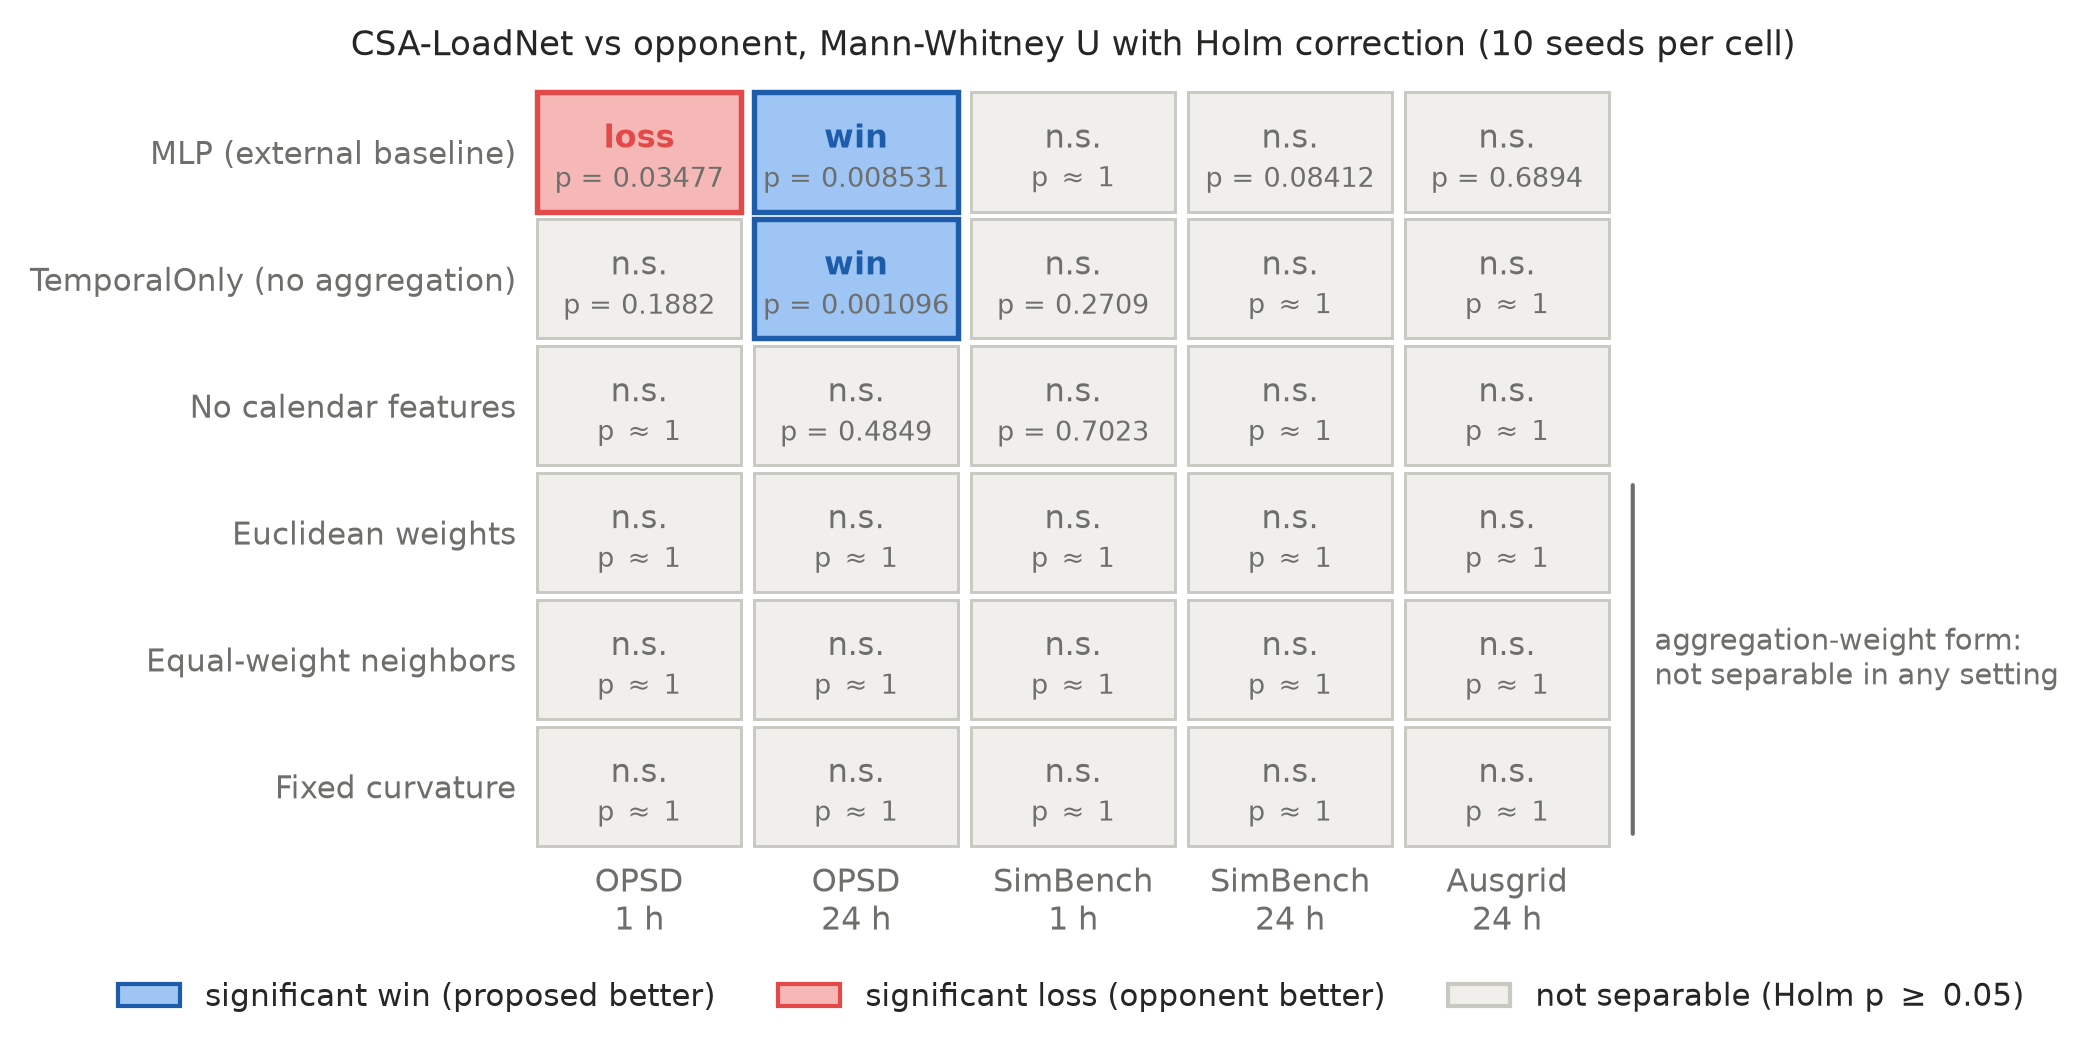
\includegraphics[width=0.94\textwidth]{figures/fig_component.png}
\caption{Proposed-versus-control decisions after scope-specific Holm correction. Fixed-split and exact-hierarchy cells use seed-level Mann--Whitney U tests with ten seeds conditional on one split. The rolling-origin cells use exact sign-flip tests over eight block means after five-seed averaging. The OPSD lead-24 fixed split contains wins against MLP and the smaller-head TemporalOnly arm; OPSD lead 1 contains a loss to MLP. The matched target-self and all tested weighting-form comparisons are unresolved in the rolling-origin primary family. The exact-hierarchy DLinear comparison is reported separately in Section 6.4.}\label{fig:3}
\end{figure*}

The matrix records why stronger controls were needed. At the OPSD fixed split, both the selected external comparison and the smaller-head TemporalOnly comparison separate. At the lead-1 settings, TemporalOnly is nominally worse than the full model but the differences are not significant (OPSD, p = 0.188; SimBench, p = 0.271). The aggregation signal is also absent at SimBench lead 24 and in the exact-hierarchy TemporalOnly comparison (p = 1 in both), with TemporalOnly nominally ahead at SimBench lead 24. No tested weight-form comparison separates after primary-family correction. Table 5 supersedes the fixed-split TemporalOnly cell for the aggregation-existence claim.

\subsection{Matched Aggregation and Weighting Controls Do Not Separate}\label{matched-aggregation-and-weighting-controls-do-not-separate}

The matched rolling-origin analysis changes the fixed-split attribution. Cross-series context has a small favorable mean relative to target-self context, but its interval crosses zero and its Holm p is 0.984. The comparison therefore does not establish that aggregation helps under the rolling-origin estimand. Weighting-form conclusions remain negative:

\begin{itemize}
\tightlist
\item
  \textbf{Poincar\'{e} vs.~Euclidean distance weights:} not separable in the rolling-origin primary family (mean MAPE difference -0.000009, Holm p = 0.984), consistent with the fixed-split nulls.
\item
  \textbf{Poincar\'{e} vs.~uniform neighbor averaging:} not separable in the rolling-origin family (mean MAPE difference -0.000066, Holm p = 0.984). Learned scores do not demonstrably improve on informative uniform cross-series context.
\item
  \textbf{Learnable vs.~fixed inverse-temperature:} fixed scale is nominally better at seven of eight origins on MAPE and all eight on WAPE. The primary MAPE result does not survive Holm correction (p = 0.0625); secondary WAPE has raw p = 0.0078 but was not multiplicity-adjusted. This is a retained adverse trend, not evidence for the learned scale and not a curvature comparison.
\end{itemize}

The joint conclusion is consequently narrower: neither the existence of cross-series context nor a learned weighting advantage is established by the matched rolling-origin primary family. The aggregation-existence conclusion comes from the matched target-self comparison; the combined uniform, Euclidean, and fixed-scale controls license only the family-level statement that no tested learned-weight advantage is established. They do not identify the best weight form or decompose the null among distance geometry and scale. Uniform neighbor averaging and target-self context are empirically competitive options, not demonstrated equivalents. The Poincar\'{e} embedding remains an implementation option rather than a supported contribution. The discrepancy with the favorable fixed split illustrates why optimization seeds on one trajectory cannot substitute for evaluation at multiple temporal blocks.

The result is specific to six OPSD series, lead 24, eight quarterly origins, and the frozen budget. Larger pools, sparser cross-correlations, or genuinely tree-structured populations might differ (Section 8). Because no equivalence margin was specified, the unresolved variants are not proven equivalent. The five-seed rolling-origin study also does not retest the MLP comparison, which remains a selected fixed-split result.

\subsection{Exact-Hierarchy Boundary: DLinear Retains the Advantage}\label{exact-hierarchy-boundary-dlinear-retains-the-advantage}

The Ausgrid experiment uses an exact hierarchy built from the 12 selected complete customers: four deterministic postcode-sorted groups each sum three leaves, and the root sums all 12. Figure 4 makes the 17-by-12 summing structure explicit; the identity \(Y=SB\) holds at every hour.

\begin{figure*}[t]
\centering
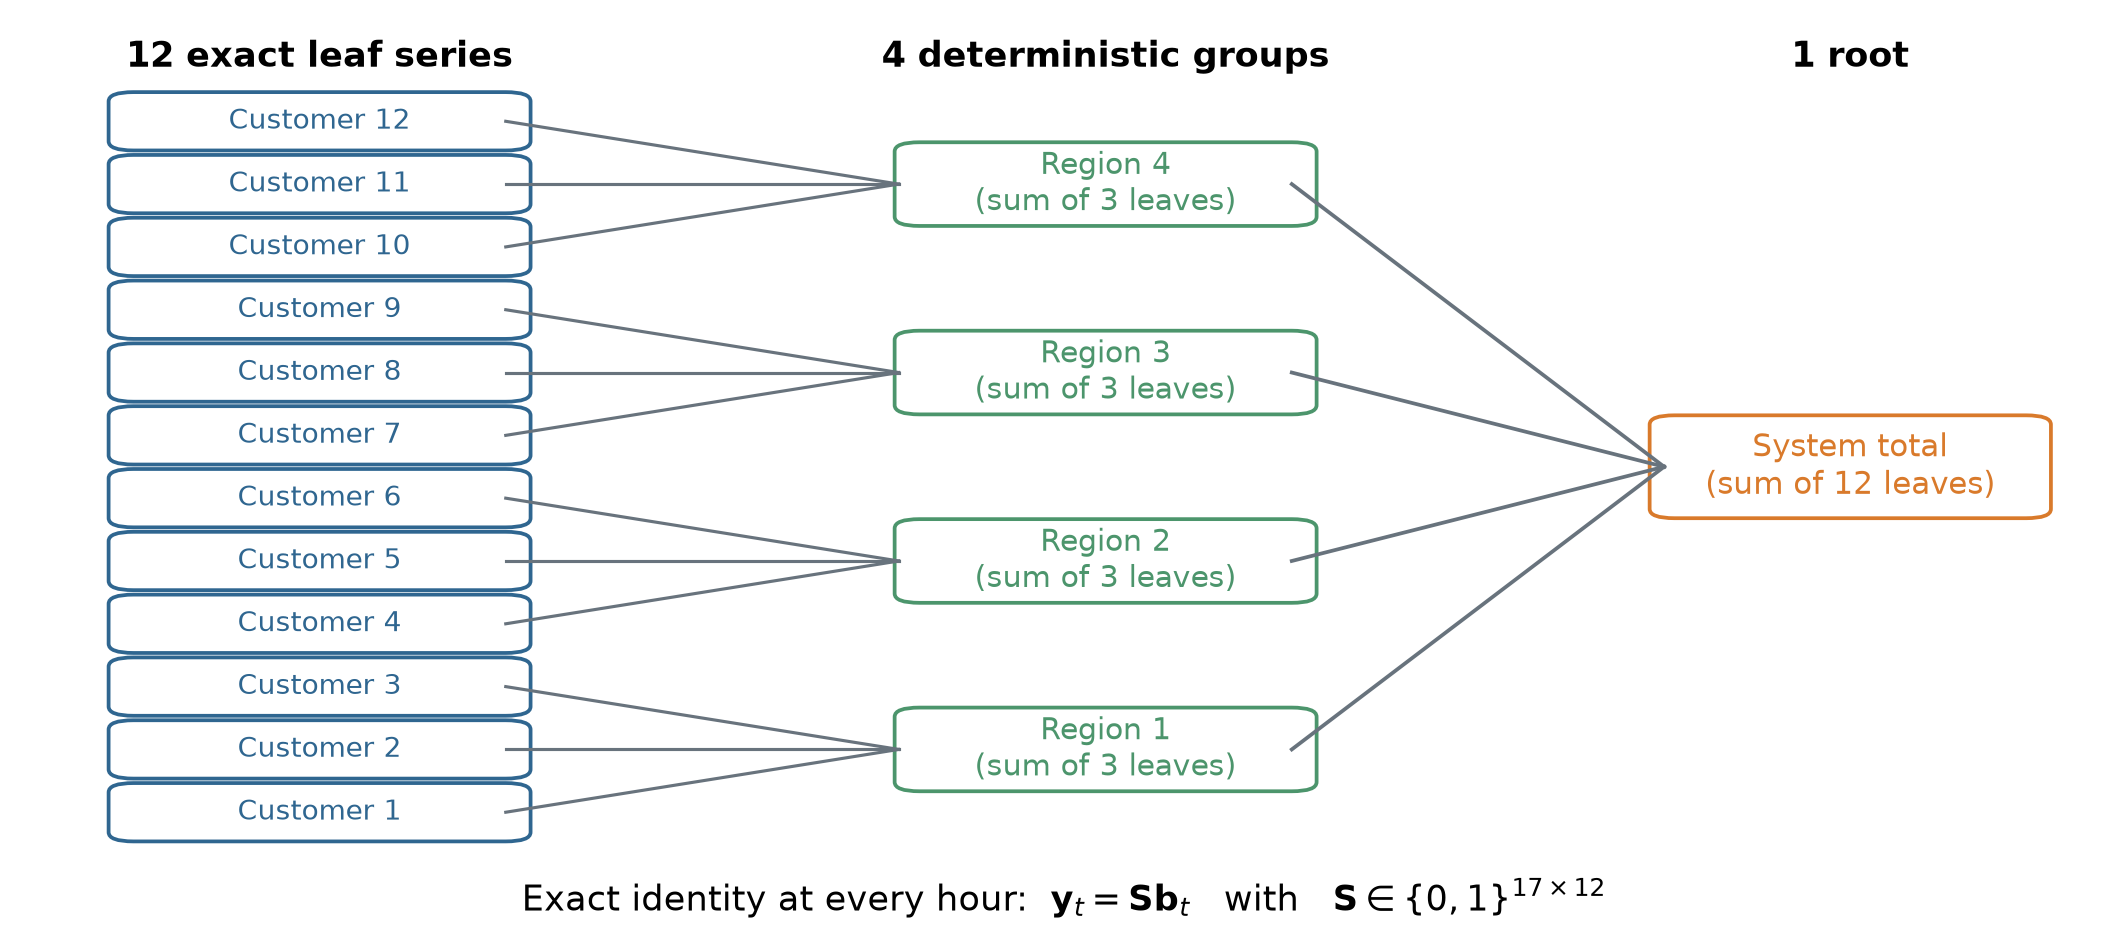
\includegraphics[width=0.94\textwidth]{figures/fig_exact_hierarchy_design.png}
\caption{Exact Ausgrid hierarchy. The four intermediate series and the system total are deterministic sums of the same 12 leaves used by every forecasting method; no outside customer enters an aggregate.}\label{fig:4}
\end{figure*}

Each trained model first produces an unreconciled matrix \(\hat Y^{\mathrm{base}}\in\mathbb R^{17\times T}\) in the node order 12 leaves, \texttt{region1}--\texttt{region4}, and \texttt{system\_total}. Let \(S\in\{0,1\}^{17\times12}\) be the fixed summing matrix shown in Figure 4. Bottom-up discards the five aggregate-node base forecasts and returns \(\hat Y^{\mathrm{BU}}=S\hat Y^{\mathrm{base}}_{1:12,:}\). Top-down computes leaf proportions \(q_\ell=\sum_{t<b}y_{\ell t}/\sum_{r=1}^{12}\sum_{t<b}y_{rt}\) from the pre-test training segment, allocates the base root forecast as \(q\hat y^{\mathrm{base}}_{17,:}\), and returns \(\hat Y^{\mathrm{TD}}=S(q\hat y^{\mathrm{base}}_{17,:})\). OLS applies the unweighted, covariance-free projection \(P=S(S^{\mathsf T}S)^{-1}S^{\mathsf T}\) independently at every forecasted timestamp: \(\hat Y^{\mathrm{OLS}}=P\hat Y^{\mathrm{base}}\). No post-reconciliation clipping or refitting is implemented. Bottom-up, top-down, and OLS are all exactly coherent by construction; only top-down estimates proportions, and it uses no test targets.

Table 6 and Figure 5 regenerate the reconciliation results from all 440 method--seed--reconciliation records. DLinear is lower-error than CSA-LoadNet under every displayed regime. DLinear with bottom-up reconciliation has the lowest mean hierarchy-weighted sMAPE (0.28017); DLinear with OLS reaches 0.28047, compared with 0.28949 for CSA-LoadNet under the same OLS projection. The 0.00902 absolute gap is a 3.22\% error increase for CSA-LoadNet when the DLinear mean is the denominator. Under OLS, CSA-LoadNet significantly loses to DLinear (Holm \(p=0.000985\)), significantly beats LSTM (\(p=0.000913\)), and is unresolved against MLP, TCN, and PatchTST-lite. The paired CSA-minus-DLinear difference is 0.00902 (pointwise 95\% bootstrap interval {[}0.00606, 0.01215{]}, paired Holm p = 0.0195). These seed-level uncertainties are conditional on the one exact-hierarchy split, and the capacity, epoch, and stride asymmetries in Section 5.2 qualify the model ranking.

\begin{table*}[t]
\centering
\footnotesize
\setlength{\tabcolsep}{3pt}
\caption{Exact-hierarchy reconciliation results regenerated in \texttt{derived\_tables/p2\_reconciliation\_summary.csv}. Values are mean $\pm$ seed standard deviation over ten seeds conditional on one fixed temporal split. Coherence violation is the mean scale-normalized structural residual; values shown as zero are exact to the reported precision.}\label{tab:6}
\begin{tabularx}{\textwidth}{@{}>{\raggedright\arraybackslash}X >{\raggedright\arraybackslash}X >{\raggedright\arraybackslash}X >{\raggedright\arraybackslash}X@{}}
\toprule
Method & Reconciliation & Hierarchy-weighted sMAPE & Mean coherence violation \\
\midrule
DLinear & Base & 0.28031 $\pm$ 0.00123 & 0.00157 \\
CSA-LoadNet & Base & 0.29051 $\pm$ 0.00467 & 0.04353 \\
DLinear & Bottom-Up & \textbf{0.28017 $\pm$ 0.00135} & 0 \\
CSA-LoadNet & Bottom-Up & 0.29140 $\pm$ 0.00466 & 0 \\
DLinear & Top-Down & 0.35971 $\pm$ 0.00078 & 0 \\
CSA-LoadNet & Top-Down & 0.36280 $\pm$ 0.00373 & 0 \\
DLinear & OLS & 0.28047 $\pm$ 0.00115 & 0 \\
CSA-LoadNet & OLS & 0.28949 $\pm$ 0.00498 & 0 \\
\bottomrule
\end{tabularx}
\end{table*}
\begin{figure*}[t]
\centering
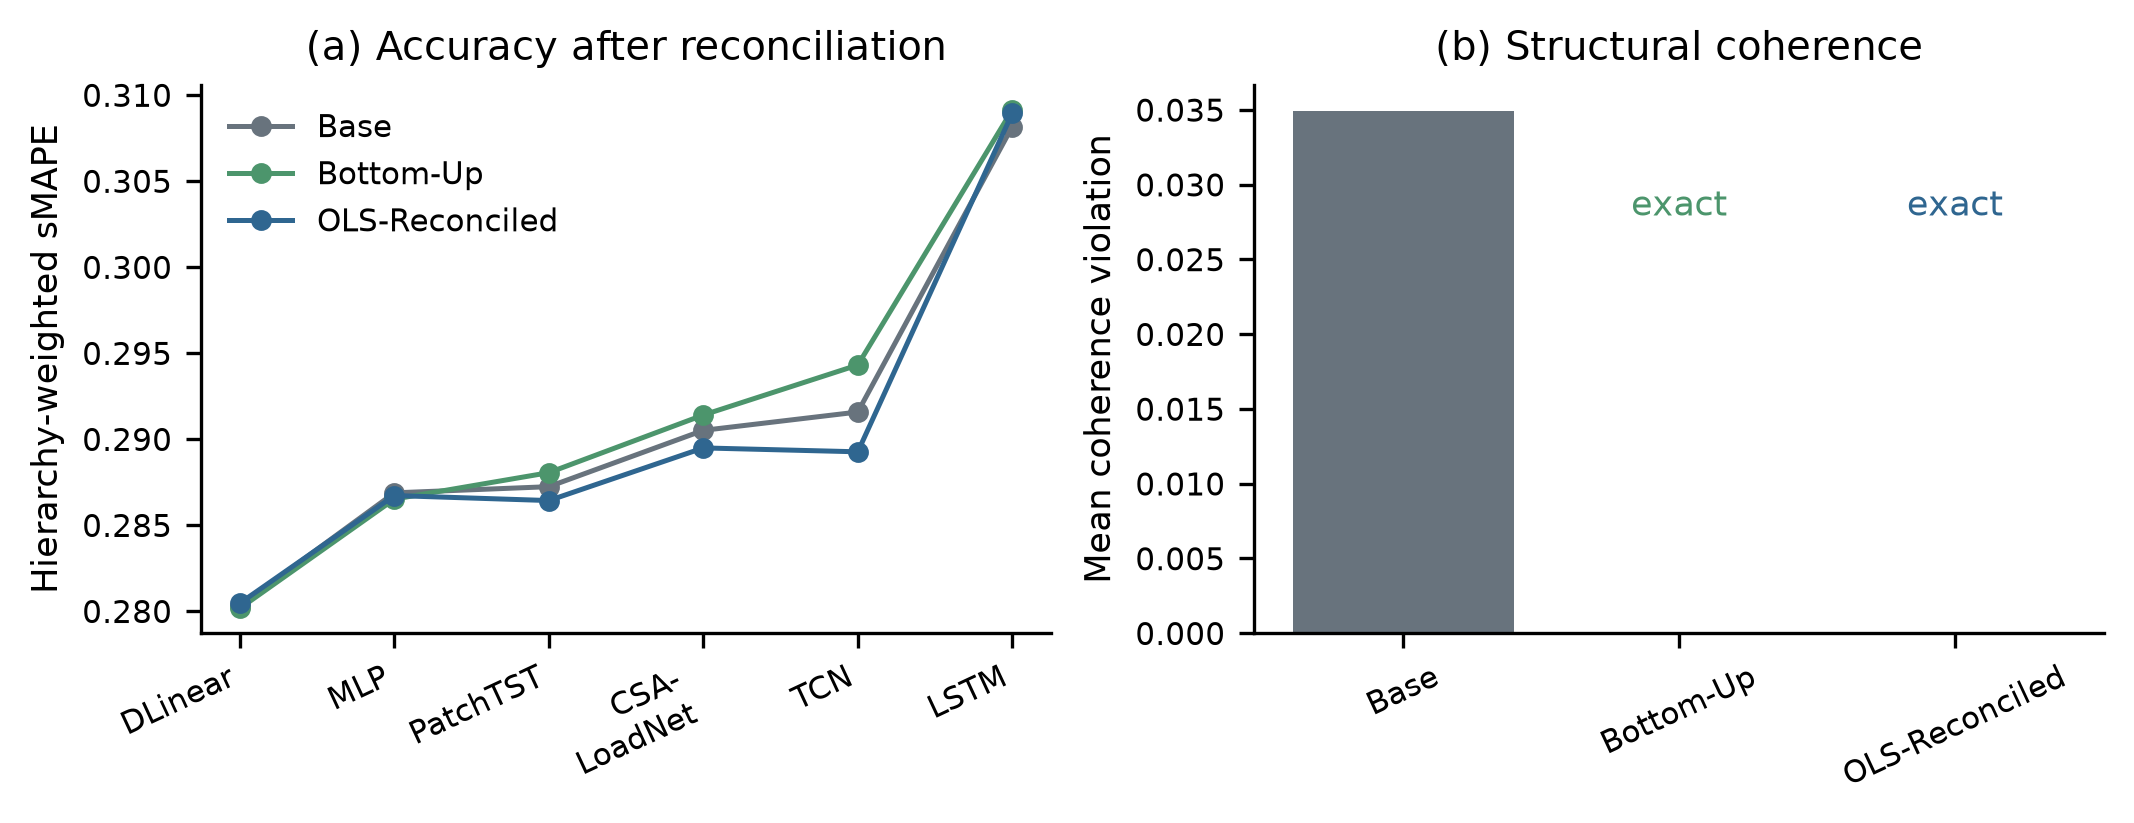
\includegraphics[width=0.94\textwidth]{figures/fig_exact_hierarchy_reconciliation.png}
\caption{(\textbf{a}) Hierarchy-weighted sMAPE under base, bottom-up, top-down, and OLS forecasts. Error bars are seed SDs conditional on the same fixed split. (\textbf{b}) Mean structural violation. Bottom-up, top-down, and OLS enforce exact coherence, but DLinear remains more accurate than CSA-LoadNet; reconciliation does not reverse the ranking.}\label{fig:5}
\end{figure*}

The result strengthens the boundary claim rather than the method claim. On the exact customer hierarchy, a strong linear decomposition with deterministic aggregation is better. Together with the rolling-origin OPSD matched-control null, the evidence does not license reserving CSA-LoadNet for any setting on the basis of an identified aggregation benefit. It does support treating coherence as a separate constraint where accounting identities matter.

\subsection{Short-Horizon and SimBench Boundaries}\label{short-horizon-and-simbench-boundaries}

The remaining cells of Figure 3 complete the boundary map. At OPSD lead 1, the MLP significantly beats CSA-LoadNet (0.010155 versus 0.010689 mean MAPE; primary Holm \(p=0.0348\)). The supplementary paired sensitivity agrees: CSA-minus-MLP MAPE is 0.000534 (pointwise 95\% CI {[}0.000248, 0.000826{]}, paired Holm \(p=0.0469\)). At this lead, recent target history may dominate the aggregation context. On SimBench, neither lead separates from the MLP. The proposed mean is only trivially lower at lead 1 (0.033349 versus 0.033385 nMAE; \(p=1\)), whereas the MLP mean is lower at lead 24 (0.058591 versus 0.060662; \(p=0.084\)). Because SimBench positions are constructed from retained quarter-hours and carry naive labels, these are lead-position results rather than guaranteed elapsed-hour effects. We therefore make no SimBench superiority or parity claim.

Figure 6 expresses six paired relative-error summaries with the denominator made explicit. For each point, the denominator is the comparator error in the same paired unit. Fixed-split and exact-hierarchy points summarize seed-paired percentages conditional on one split; the rolling-origin point summarizes eight block-paired percentages after five-seed averaging. Positive values favor CSA-LoadNet. Only the selected OPSD lead-24 fixed-split comparison combines a positive mean effect with corrected significance. OPSD lead 1, SimBench lead 24, and exact-hierarchy Ausgrid favor the named comparators; SimBench lead 1 is near zero. The rolling-origin percentage is descriptive and does not replace the block-level test in Table 5.

\begin{figure*}[t]
\centering
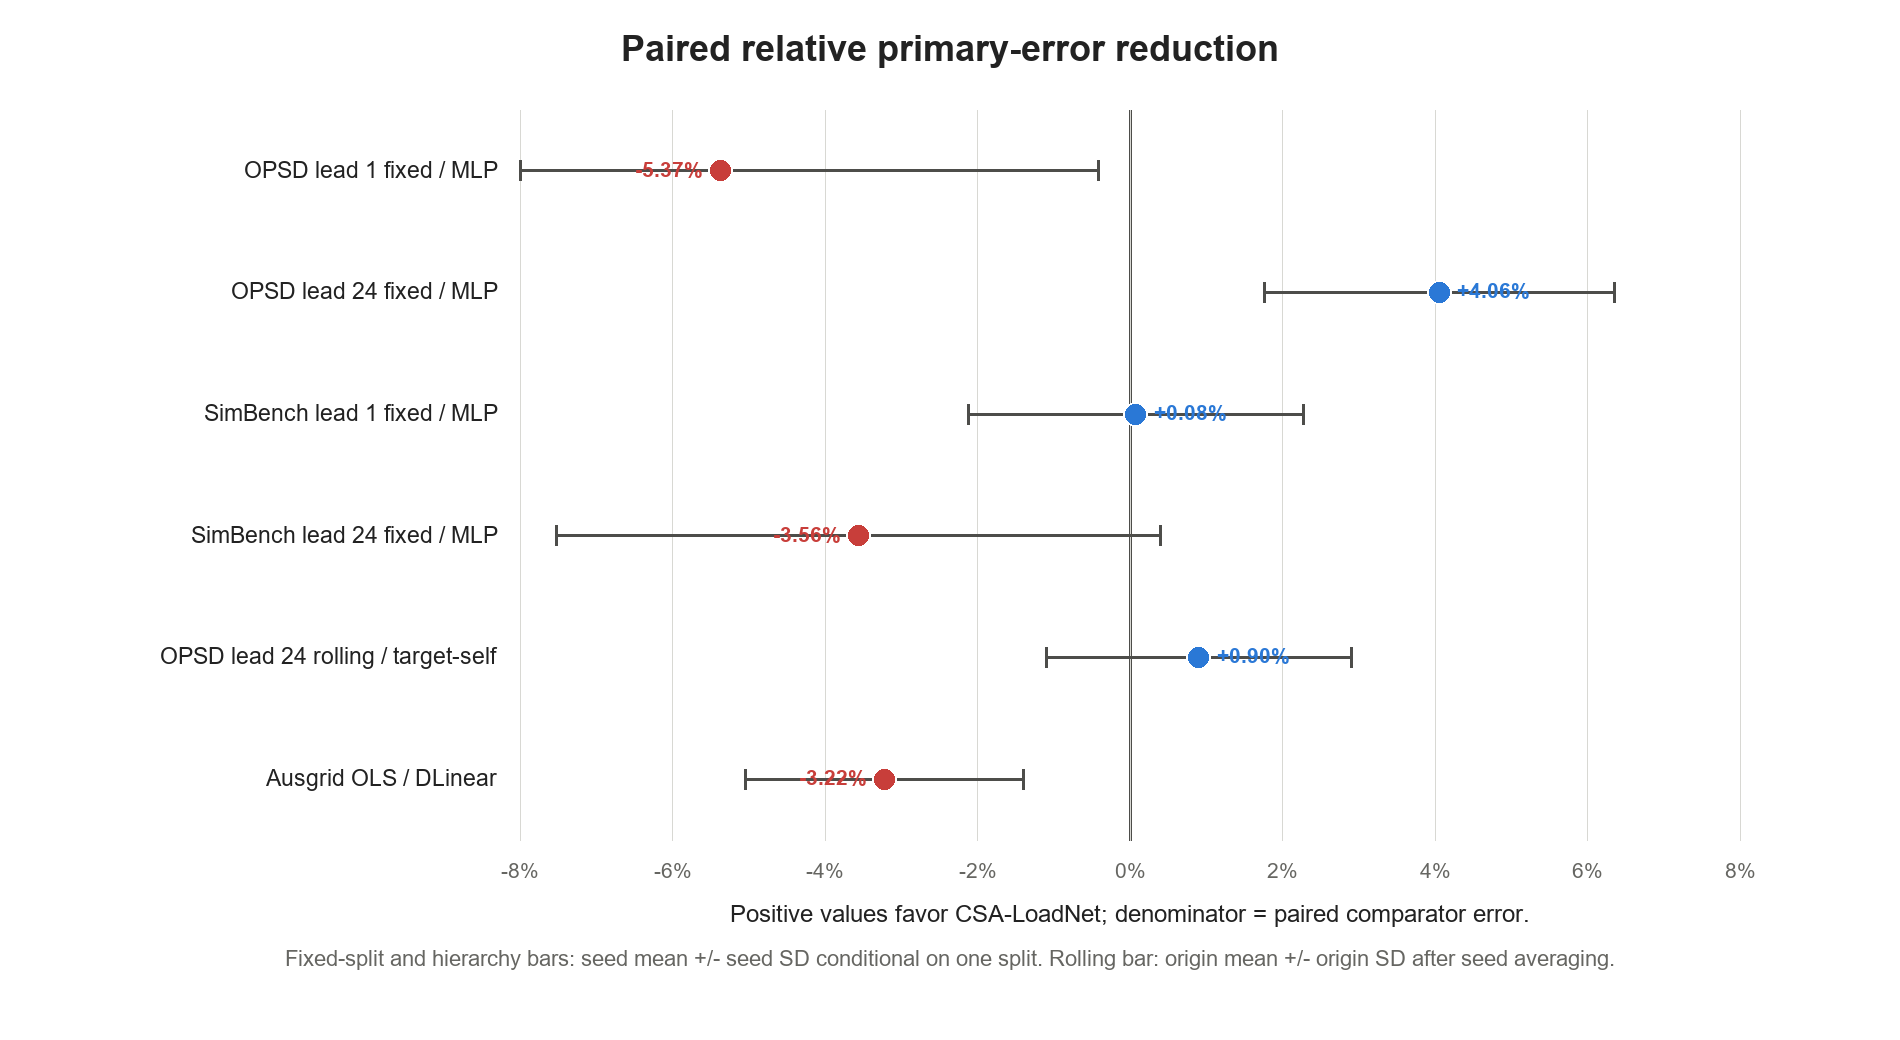
\includegraphics[width=0.94\textwidth]{figures/fig_cross_dataset_effects.png}
\caption{Paired relative reduction in each setting's primary error for CSA-LoadNet against the named comparator. Points show means and error bars show standard deviations. Fixed-split and hierarchy error bars represent seed variation conditional on one split; the rolling-origin error bar represents variation across eight block means after seed averaging. Positive values favor CSA-LoadNet. Percentages use the paired comparator error as denominator and are descriptive effect displays, not the test statistic.}\label{fig:6}
\end{figure*}

\subsection{Cross-Setting Rank and Compute Profiles}\label{cross-setting-rank-and-compute-profiles}

Figure 7 reports current ranks for six scope-specific rosters. CSA-LoadNet ranks 5/7 on OPSD lead 1, 4/7 on the OPSD lead-24 fixed split, 2/6 in the rolling-origin control family, 2/7 and 5/7 on the two SimBench fixed splits, and 6/11 on the exact hierarchy under common OLS reconciliation. These ranks describe mean ordering only; they do not override the corrected decisions. Missing cells are not imputed, each denominator is printed in the figure, and no cross-dataset average rank is formed because the metrics and method rosters differ.

\begin{figure*}[t]
\centering
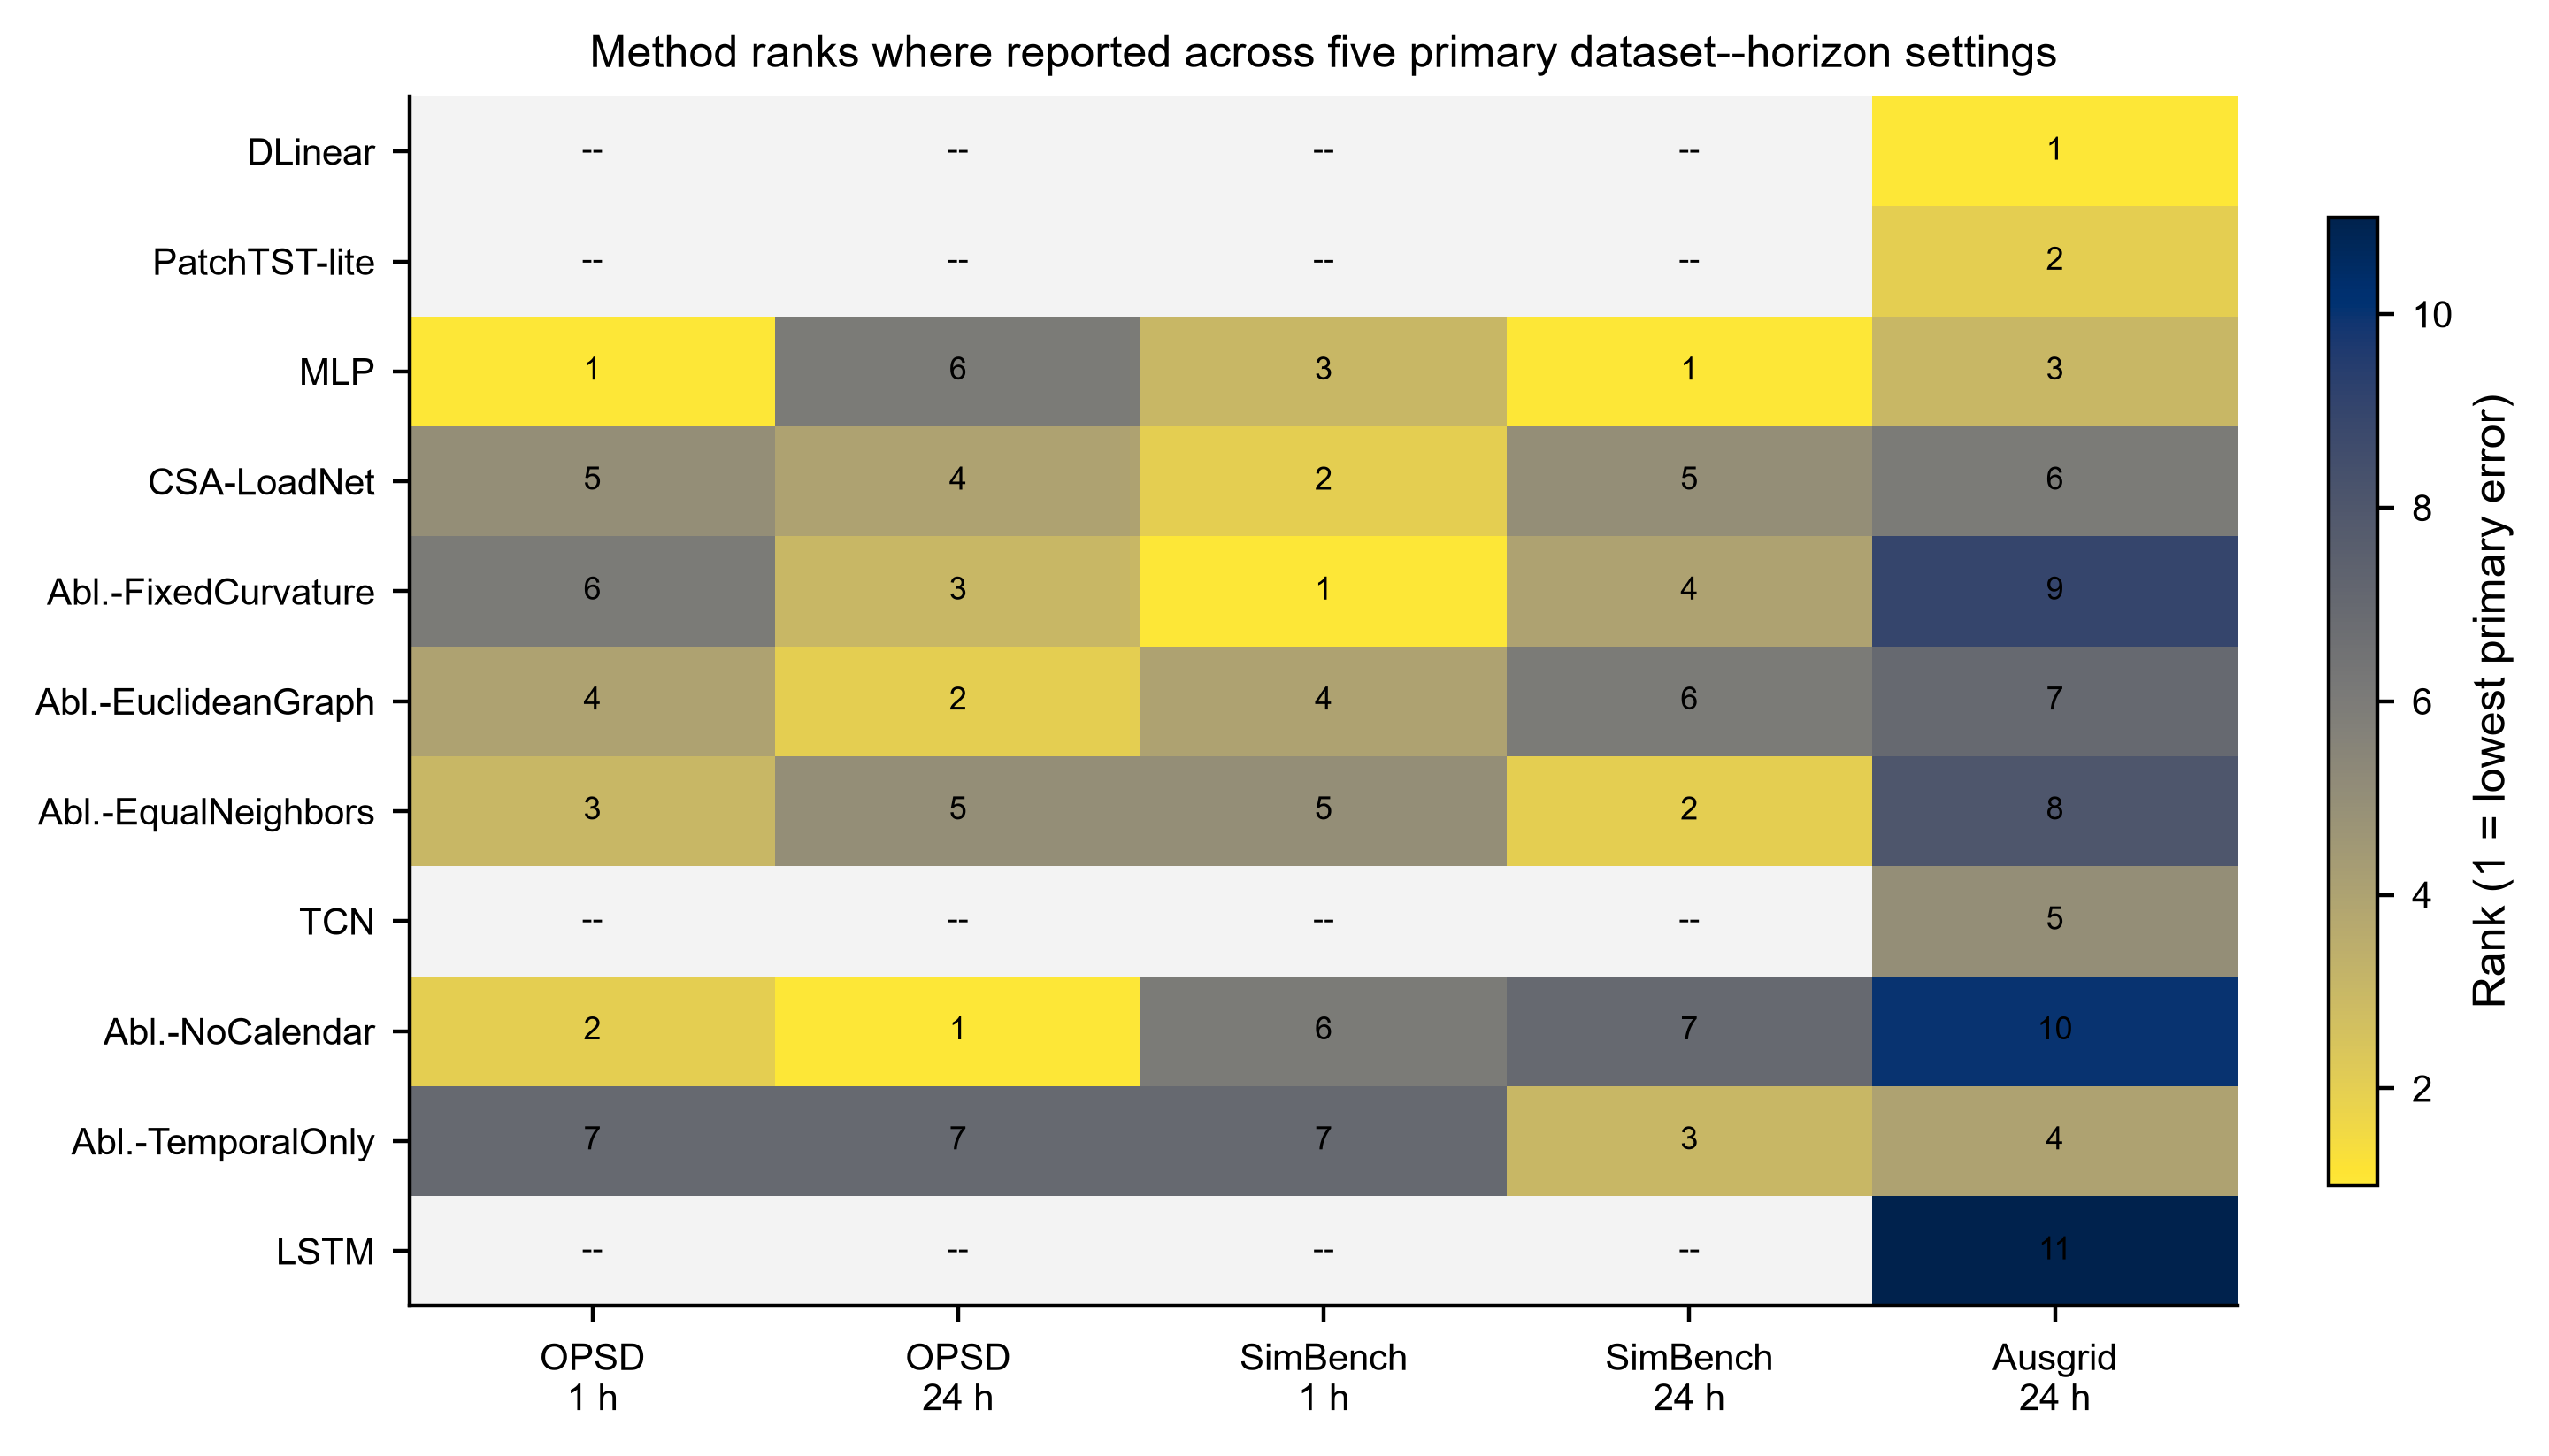
\includegraphics[width=0.94\textwidth]{figures/fig_cross_setting_ranks.png}
\caption{Ranks by scope-specific primary error, regenerated in \texttt{derived\_tables/p2\_cross\_setting\_ranks.csv}. Rank 1 is the lowest mean error within a column; each cell reports rank/roster size. Dashes mark methods absent from an experiment. Fixed-split columns use ten-seed means conditional on one split, the rolling column uses means across eight block means, and the Ausgrid column uses the exact hierarchy with OLS reconciliation.}\label{fig:7}
\end{figure*}

The run-time profile in Figure 8 supplies the computational counterpart. It places each CSA-LoadNet setting on a logarithmic runtime axis and annotates the dataset-specific primary error. The vertical lanes separate settings and have no quantitative scale; annotated error values use different metrics and must not be compared across datasets.

\begin{figure*}[t]
\centering
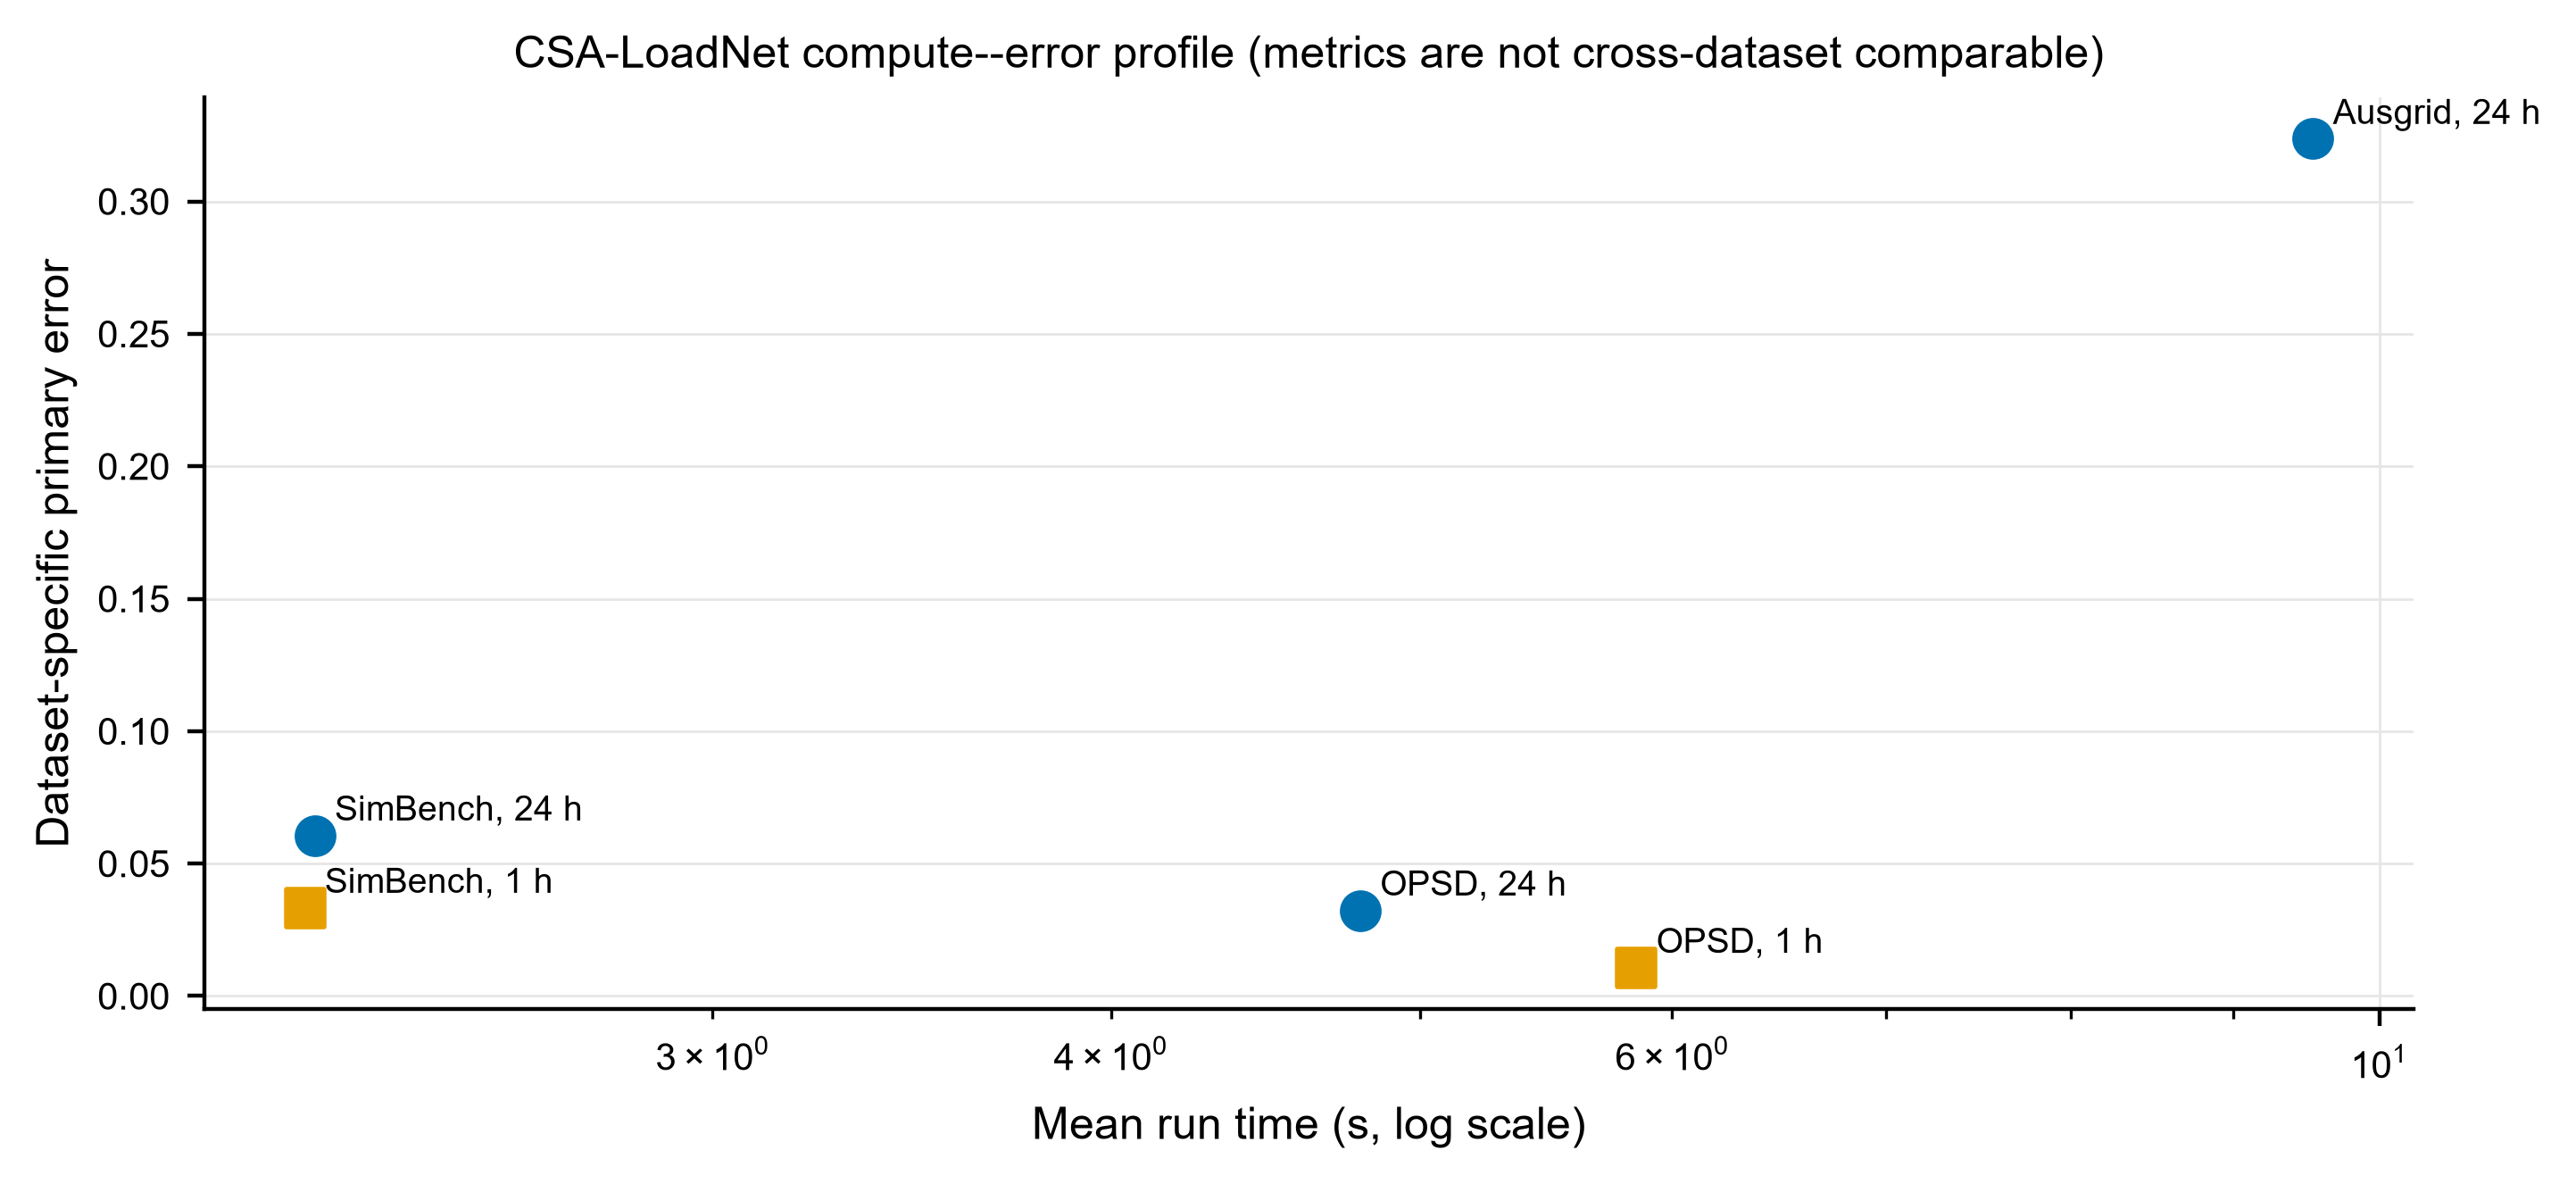
\includegraphics[width=0.94\textwidth]{figures/fig_compute_error_profile.png}
\caption{Mean wall-clock time and annotated dataset-specific primary error for CSA-LoadNet at each evaluated horizon. The x-axis is logarithmic; vertical placement is categorical. Timings are interpreted within dataset and execution environment, not across CPU and GPU blocks.}\label{fig:8}
\end{figure*}

\begin{table*}[t]
\centering
\footnotesize
\setlength{\tabcolsep}{3pt}
\caption{Stability summary across the complete primary-metric comparisons. "Supported" requires Holm-adjusted $p<0.05$; a nominal mean ordering without corrected separation is not counted. Percentages use the named comparator mean as denominator.}\label{tab:7}
\begin{tabularx}{\textwidth}{@{}>{\raggedright\arraybackslash}X >{\raggedright\arraybackslash}X >{\raggedright\arraybackslash}X >{\raggedright\arraybackslash}X@{}}
\toprule
Setting & Proposed mean position & Corrected decision against named comparator & Interpretation \\
\midrule
OPSD, lead 1 fixed split & Rank 5/7; 5.26\% higher mean MAPE than MLP & Significant loss & Short-horizon boundary; seed inference conditional on one split \\
OPSD, lead 24 fixed split & Rank 4/7; 4.07\% lower mean MAPE than selected MLP & Significant win & Selected-comparator result on one split \\
OPSD, lead 24 rolling blocks & Rank 2/6; 0.69\% lower mean MAPE than matched target-self & Not separable & Aggregation-existence claim not confirmed \\
SimBench, lead 1 fixed split & Rank 2/7; 0.11\% lower mean normalized MAE than MLP & Not separable & No superiority or equivalence claim \\
SimBench, lead 24 fixed split & Rank 5/7; 3.53\% higher mean normalized MAE than MLP & Not separable & Adverse nominal ordering \\
Ausgrid, lead 24 exact hierarchy & Rank 6/11; 3.22\% higher mean hierarchy-weighted sMAPE than DLinear under OLS & Significant loss & Coherence achieved; no accuracy-superiority claim \\
\bottomrule
\end{tabularx}
\end{table*}

The table and rank profile separate two levels of evidence. The selected MLP comparison remains favorable on one fixed split, but cross-series aggregation does not separate from the capacity-matched target-self control over eight rolling blocks. The tested attention parameterizations likewise remain unresolved. The evidence supports a component-evaluation result, not an aggregation-performance claim.

\begin{center}\rule{0.5\linewidth}{0.5pt}\end{center}

\section{Discussion}\label{discussion}

\subsection{Aggregation, Weighting, and Hierarchical Coherence}\label{aggregation-weighting-and-hierarchical-coherence}

The ten-seed fixed split favors CSA-LoadNet over the smaller-head TemporalOnly arm and the selected MLP. In the matched rolling-origin analysis, CSA-LoadNet's mean MAPE is only 0.69\% lower than target-self context when the target-self mean is the denominator, and the Holm-adjusted p is 0.984. Learned Poincar\'{e}, uniform, and Euclidean cross-series weighting also do not separate. The fixed-scale arm is nominally best, including lower WAPE at every origin, but its primary MAPE p becomes 0.0625 after correction. The architecture screen and the single favorable fixed split therefore cannot carry a confirmatory aggregation claim.

The exact Ausgrid experiment answers a different question. It constructs all four regional aggregates and the root from the same 12 leaves and applies common reconciliation transformations to every method. Bottom-up and OLS reconciliation remove structural violations, yet DLinear remains more accurate than CSA-LoadNet. Coherence is therefore a constraint that can be enforced after forecasting; it is not evidence that the underlying forecaster is accurate.

Taken together, the experiments locate uncertainty rather than a benefit. Pool context is not separated from a matched target-only context over the evaluated OPSD origins, and additional weighting complexity is unsupported. The shared encoder outperforms the parameter-matched independent arm, but that control changes hidden widths and arithmetic, so sharing itself remains unresolved. Independently repeated weather years and a compute-matched independent encoder would be needed to test either mechanism more cleanly.

\subsection{Horizon Interpretation Remains Unresolved}\label{horizon-interpretation-remains-unresolved}

The fixed-split horizon asymmetry admits a hypothesis but not a demonstrated mechanism. At lead 1, each country's own recent observations may contain most recoverable information; at lead 24, synchronized daily and weekly shapes could supply useful context. However, the lead-24 matched rolling-origin comparison does not establish a context benefit, and the rolling-origin study did not evaluate lead 1. Because no weather variables or mechanism intervention links the series, the study does not claim why errors differ by horizon.

\subsection{Implications for the Cross-Series Forecasting Literature}\label{implications-for-the-cross-series-forecasting-literature}

Our results neither reject cross-series modeling nor support an aggregation or weighting advantage. On the fixed split, CSA-LoadNet's mean MAPE is 6.49\% lower than the smaller-head TemporalOnly mean, using TemporalOnly as the denominator. Across rolling-origin blocks, it is only 0.69\% lower than the matched target-self mean, using target-self as the denominator, and the contrast is unresolved. No primary-family weighting-form difference is established; equivalence within a prespecified tolerance was not tested. This discrepancy shows why mechanism claims require both matched component controls and evaluation at multiple temporal blocks. Runtime evidence is interpreted only within a common execution environment.

\begin{center}\rule{0.5\linewidth}{0.5pt}\end{center}

\section{Limitations}\label{limitations}

\begin{enumerate}
\def\labelenumi{\arabic{enumi}.}
\tightlist
\item
  \textbf{No aggregation superiority claim survives the matched temporal analysis.} The fixed split favors CSA-LoadNet over the selected MLP and smaller-head TemporalOnly arms, but the matched target-self contrast over eight rolling blocks is unresolved (MAPE Holm \(p=0.984\); secondary WAPE raw \(p=0.227\)). The experiment predicts one scalar at lead 24 and does not score a 24-point next-day trajectory. The OPSD lead-1 comparison favors MLP, and neither SimBench lead separates from MLP.
\item
  \textbf{The method does not transfer to the exact customer/region/system hierarchy as implemented.} Under common OLS reconciliation, CSA-LoadNet significantly loses to DLinear (Holm \(p<0.001\)), while its contrasts against MLP, TCN, and PatchTST-lite remain unresolved under the primary family. Bottom-up, top-down, and OLS reconciliation satisfy the accounting identities, but coherence does not establish forecaster accuracy. MinT with covariance shrinkage and end-to-end coherence-constrained training remain untested.
\item
  \textbf{The weight-form inseparability is a bounded negative.} Learned Poincar\'{e} weighting does not separate from uniform or Euclidean context in the rolling-origin primary family, consistent with fixed-split nulls across pools of 6, 8, and 17 series. Fixed scale is nominally better in the rolling-origin study (MAPE Holm \(p=0.0625\); secondary WAPE raw \(p=0.0078\)), so the data do not favor learned scaling. No equivalence margin was specified.
\item
  \textbf{Only the rolling-origin shared-encoder component arms are parameter- and head-matched.} External-model counts range from 338 to 70,597 and epoch budgets differ. On Ausgrid, CSA variants use stride 6 while external baselines use stride 3, so the methods receive unequal training-example exposure. The independent-encoder arm matches total parameters but changes hidden widths and uses substantially less encoder arithmetic. Neither the fixed-split rankings nor the shared-encoder contrast is a fully capacity-and-compute-controlled causal comparison.
\item
  \textbf{Ausgrid structural selection sees the full record.} The completeness filter and top-energy leaf ranking use all three years before the chronological split. This does not train model parameters on test targets, but it is not a train-only selection design and may favor continuous, high-consumption customers. Only one deterministic grouping is tested.
\item
  \textbf{Timestamp and missingness handling are limited.} OPSD is kept in UTC, whereas SimBench and constructed Ausgrid labels have no represented timezone and receive no daylight-saving adjustment. Sequence-phase covariates come from row indices rather than parsed timestamps. The rolling-origin OPSD audit records 43 discarded source rows before reaching 35,000 retained rows, so a 24-position lead is not always 24 elapsed UTC hours around gaps. SimBench discard counts remain unavailable, and Ausgrid blank half-hours are set to zero. Sensitivity to these choices is untested.
\item
  \textbf{Multi-block evidence remains within one observed record.} The eight quarterly blocks span 2017--2018 and use the same six country series. Their 672-origin test blocks are disjoint, but they are not independent weather-year or system replications: the series are shared and later training histories contain earlier observations. The exact sign-flip test therefore relies on sign-exchangeability of block-level paired differences rather than proven block independence. MLP selection used the fixed test trajectory and was excluded from the rolling-origin confirmatory family.
\item
  \textbf{No exogenous weather or operational covariates are used.} All models forecast from load history and four row-index phase features. Weather-aware extensions, holidays, localized civil time, dispatch consequences, and deployment remain untested.
\item
  \textbf{The rolling-origin experiment has not been independently replicated.} The accepted records, frozen configuration, origin tables, and analysis code are retained in the supplementary evidence, but a separately executed replication remains unavailable.
\end{enumerate}

\begin{center}\rule{0.5\linewidth}{0.5pt}\end{center}

\section{Conclusions}\label{conclusions}

This study tests which components of the CSA-LoadNet cross-series attention baseline remain supported after capacity matching and evaluation at multiple temporal blocks. CSA-LoadNet is not a GCN or HGCN, so these results do not test the graph-convolutional method named in the locked title. The OPSD fixed split favors CSA-LoadNet over a selected MLP and a smaller-head TemporalOnly arm, but the eight-block analysis does not separate it from a matched target-self context: mean MAPE is 0.036640 versus 0.036894 (Holm \(p=0.984\)), and mean WAPE is 0.036775 versus 0.037109 (raw \(p=0.227\)). The fixed-split aggregation attribution is therefore not confirmed under the rolling-origin estimand.

The form of the aggregation weights is likewise unsupported as a differentiator. Learned Poincar\'{e} weights do not separate from uniform or Euclidean context after correction, and fixed scaling is nominally better rather than worse. The shared encoder beats the parameter-matched independent arm, but width allocation and arithmetic differ, precluding a sharing claim. OPSD lead-1 and SimBench findings remain adverse or unresolved. On the exact hierarchy under common OLS reconciliation, DLinear retains the accuracy advantage: CSA-LoadNet's mean error is 3.22\% higher using DLinear's mean as the denominator (Holm \(p=0.000985\)). Reconciliation supplies coherence, not accuracy superiority. The resulting contribution is a matched null result, an empirical limit on weighting complexity, and a separation between forecast accuracy and structural coherence.

\begin{center}\rule{0.5\linewidth}{0.5pt}\end{center}

\section*{Author Contributions}

{[}AUTHOR INPUT REQUIRED: assign verified CRediT roles to Zheng Jieyun, Zhang Linyao, Zhang Zhanghuang, Chen Zhuolin, and Shi Ying; obtain every author's approval; and insert the author-approved responsibility statement.{]}

\section*{Funding}

{[}AUTHOR INPUT REQUIRED: insert the verified funder, grant number, and APC funder, or state ``This research received no external funding.''{]}

\section*{Institutional Review Board Statement}

Not applicable.

\section*{Informed Consent Statement}

Not applicable.

\section*{Data Availability Statement}

All datasets used in this study are public: the Open Power System Data 60 min package (https://open-power-system-data.org) {[}29{]}, SimBench load profiles (https://simbench.de) {[}30{]}, and Ausgrid solar-home electricity data (https://www.ausgrid.com.au) {[}24{]}. The supplementary package contains the CSA-LoadNet implementation and configurations; 280 fixed-split non-hierarchical decision-set records; 440 exact-hierarchy model--reconciliation records; and the accepted rolling-origin evidence comprising 240 method--block--seed rows, 6,750 date-aggregated forecast-target audit rows, block-level inference, and a validation report. {[}AUTHOR INPUT REQUIRED: confirm the package-access wording and deposit a persistent public archive before adding a repository URL or DOI.{]} No persistent public archive is verified in the current evidence.

\section*{Acknowledgments}

{[}AUTHOR INPUT REQUIRED: confirm the final acknowledgment and venue-compliant generative-AI disclosure, including the tool, purposes, author review, and responsibility statement.{]} The internal preparation record indicates use of Claude (Anthropic) for language drafting and editing and for assistance with analysis and figure-generation code, but author approval of the submission wording is not verified in this worktree.

\section*{Conflicts of Interest}

{[}AUTHOR INPUT REQUIRED: insert the author-confirmed conflict-of-interest statement.{]}

\begin{center}\rule{0.5\linewidth}{0.5pt}\end{center}

\begin{thebibliography}{99}
\bibitem{ref1} Li, J.; Li, J.; Li, J.; Zhang, G. Bayesian-Optimized GCN-BiLSTM-Adaboost Model for Power-Load Forecasting. \emph{Electronics} \textbf{2025}, \emph{14}(16), 3332. \url{https://doi.org/10.3390/electronics14163332}
\bibitem{ref2} Zhou, H.; Ai, Q.; Li, R. Short-Term Multi-Energy Load Forecasting Method Based on Transformer Spatio-Temporal Graph Neural Network. \emph{Energies} \textbf{2025}, \emph{18}(17), 4466. \url{https://doi.org/10.3390/en18174466}
\bibitem{ref3} Wu, M.; Feng, W.; Li, X.; Liu, Y.; Cao, C. Short-Term Power Load Forecasting Using an Improved Model Integrating GCN and Transformer. \emph{Applied Sciences} \textbf{2025}, \emph{15}(13), 7003. \url{https://doi.org/10.3390/app15137003}
\bibitem{ref4} Zhang, J.; Yu, B.; Lai, H.; Liu, L.; Zhou, J.; Lou, F.; Ni, Y.; Peng, Y.; Yu, Z. LoadSeer: Exploiting Tensor Graph Convolutional Network for Power Load Forecasting With Spatio-Temporal Characteristics. \emph{IEEE Access} \textbf{2024}, \emph{12}, 190337--190346. \url{https://doi.org/10.1109/ACCESS.2024.3514174}
\bibitem{ref5} Zeng, A.; Chen, M.; Zhang, L.; Xu, Q. Are Transformers Effective for Time Series Forecasting? \emph{Proceedings of the AAAI Conference on Artificial Intelligence} \textbf{2023}, \emph{37}(9), 11121--11128. \url{https://doi.org/10.1609/aaai.v37i9.26317}
\bibitem{ref6} Makridakis, S.; Spiliotis, E.; Assimakopoulos, V. Statistical and Machine Learning forecasting methods: Concerns and ways forward. \emph{PLOS ONE} \textbf{2018}, \emph{13}(3), e0194889. \url{https://doi.org/10.1371/journal.pone.0194889}
\bibitem{ref7} Makridakis, S.; Spiliotis, E.; Assimakopoulos, V. The M4 Competition: 100,000 time series and 61 forecasting methods. \emph{International Journal of Forecasting} \textbf{2020}, \emph{36}(1), 54--74. \url{https://doi.org/10.1016/j.ijforecast.2019.04.014}
\bibitem{ref8} Hewamalage, H.; Ackermann, K.; Bergmeir, C. Forecast evaluation for data scientists: common pitfalls and best practices. \emph{Data Mining and Knowledge Discovery} \textbf{2023}, \emph{37}(2), 788--832. \url{https://doi.org/10.1007/s10618-022-00894-5}
\bibitem{ref9} Hochreiter, S.; Schmidhuber, J. Long Short-Term Memory. \emph{Neural Computation} \textbf{1997}, \emph{9}(8), 1735--1780. \url{https://doi.org/10.1162/neco.1997.9.8.1735}
\bibitem{ref10} Kong, W.; Dong, Z.Y.; Jia, Y.; Hill, D.J.; Xu, Y.; Zhang, Y. Short-Term Residential Load Forecasting Based on LSTM Recurrent Neural Network. \emph{IEEE Transactions on Smart Grid} \textbf{2019}, \emph{10}(1), 841--851. \url{https://doi.org/10.1109/TSG.2017.2753802}
\bibitem{ref11} Salinas, D.; Flunkert, V.; Gasthaus, J.; Januschowski, T. DeepAR: Probabilistic forecasting with autoregressive recurrent networks. \emph{International Journal of Forecasting} \textbf{2020}, \emph{36}(3), 1181--1191. \url{https://doi.org/10.1016/j.ijforecast.2019.07.001}
\bibitem{ref12} Lara-Ben\'{\i}tez, P.; Carranza-Garc\'{\i}a, M.; Luna-Romera, J.M.; Riquelme, J.C. Temporal Convolutional Networks Applied to Energy-Related Time Series Forecasting. \emph{Applied Sciences} \textbf{2020}, \emph{10}(7), 2322. \url{https://doi.org/10.3390/app10072322}
\bibitem{ref13} Lim, B.; Ar\i{}k, S.\"{O}.; Loeff, N.; Pfister, T. Temporal Fusion Transformers for interpretable multi-horizon time series forecasting. \emph{International Journal of Forecasting} \textbf{2021}, \emph{37}(4), 1748--1764. \url{https://doi.org/10.1016/j.ijforecast.2021.03.012}
\bibitem{ref14} Zhou, H.; Zhang, S.; Peng, J.; Zhang, S.; Li, J.; Xiong, H.; Zhang, W. Informer: Beyond Efficient Transformer for Long Sequence Time-Series Forecasting. \emph{Proceedings of the AAAI Conference on Artificial Intelligence} \textbf{2021}, \emph{35}(12), 11106--11115. \url{https://doi.org/10.1609/aaai.v35i12.17325}
\bibitem{ref15} Zhao, X.; Peng, H.; Zhang, L.; Ma, H. Research on a Short-Term Power Load Forecasting Method Based on a Three-Channel LSTM-CNN. \emph{Electronics} \textbf{2025}, \emph{14}(11), 2262. \url{https://doi.org/10.3390/electronics14112262}
\bibitem{ref16} Xu, J.; Zhang, L.; Zhang, Z. Research on BiLSTM--Transformer Power Load Forecasting Method Based on Dynamic Adaptive Fusion. \emph{Energies} \textbf{2026}, \emph{19}(6), 1473. \url{https://doi.org/10.3390/en19061473}
\bibitem{ref17} Yang, M.; Chen, Y.; Fang, G.; Ma, C.; Liu, Y.; Wang, J. A Short-Term Power Load Forecasting Method Based on SBOA--SVMD-TCN--BiLSTM. \emph{Electronics} \textbf{2024}, \emph{13}(17), 3441. \url{https://doi.org/10.3390/electronics13173441}
\bibitem{ref18} Dakheel, F.; \c{C}evik, M. Optimizing Smart Grid Load Forecasting via a Hybrid Long Short-Term Memory-XGBoost Framework: Enhancing Accuracy, Robustness, and Energy Management. \emph{Energies} \textbf{2025}, \emph{18}(11), 2842. \url{https://doi.org/10.3390/en18112842}
\bibitem{ref19} Lai, G.; Chang, W.-C.; Yang, Y.; Liu, H. Modeling Long- and Short-Term Temporal Patterns with Deep Neural Networks. In Proceedings of the 41st International ACM SIGIR Conference on Research \& Development in Information Retrieval, 2018; pp. 95--104. \url{https://doi.org/10.1145/3209978.3210006}
\bibitem{ref20} Yu, B.; Yin, H.; Zhu, Z. Spatio-Temporal Graph Convolutional Networks: A Deep Learning Framework for Traffic Forecasting. In Proceedings of the Twenty-Seventh International Joint Conference on Artificial Intelligence (IJCAI-18), 2018; pp. 3634--3640. \url{https://doi.org/10.24963/ijcai.2018/505}
\bibitem{ref21} Wu, Z.; Pan, S.; Long, G.; Jiang, J.; Chang, X.; Zhang, C. Connecting the Dots: Multivariate Time Series Forecasting with Graph Neural Networks. In Proceedings of the 26th ACM SIGKDD International Conference on Knowledge Discovery \& Data Mining, 2020; pp. 753--763. \url{https://doi.org/10.1145/3394486.3403118}
\bibitem{ref22} Hyndman, R.J.; Ahmed, R.A.; Athanasopoulos, G.; Shang, H.L. Optimal combination forecasts for hierarchical time series. \emph{Computational Statistics \& Data Analysis} \textbf{2011}, \emph{55}(9), 2579--2589. \url{https://doi.org/10.1016/j.csda.2011.03.006}
\bibitem{ref23} Wickramasuriya, S.L.; Athanasopoulos, G.; Hyndman, R.J. Optimal Forecast Reconciliation for Hierarchical and Grouped Time Series Through Trace Minimization. \emph{Journal of the American Statistical Association} \textbf{2019}, \emph{114}(526), 804--819. \url{https://doi.org/10.1080/01621459.2018.1448825}
\bibitem{ref24} Ratnam, E.L.; Weller, S.R.; Kellett, C.M.; Murray, A.T. Residential load and rooftop PV generation: an Australian distribution network dataset. \emph{International Journal of Sustainable Energy} \textbf{2017}, \emph{36}(8), 787--806. \url{https://doi.org/10.1080/14786451.2015.1100196}
\bibitem{ref25} Tashman, L.J. Out-of-sample tests of forecasting accuracy: an analysis and review. \emph{International Journal of Forecasting} \textbf{2000}, \emph{16}(4), 437--450. \url{https://doi.org/10.1016/S0169-2070(00})00065-0
\bibitem{ref26} Bergmeir, C.; Ben\'{\i}tez, J.M. On the use of cross-validation for time series predictor evaluation. \emph{Information Sciences} \textbf{2012}, \emph{191}, 192--213. \url{https://doi.org/10.1016/j.ins.2011.12.028}
\bibitem{ref27} Hyndman, R.J.; Koehler, A.B. Another look at measures of forecast accuracy. \emph{International Journal of Forecasting} \textbf{2006}, \emph{22}(4), 679--688. \url{https://doi.org/10.1016/j.ijforecast.2006.03.001}
\bibitem{ref28} Diebold, F.X.; Mariano, R.S. Comparing Predictive Accuracy. \emph{Journal of Business \& Economic Statistics} \textbf{1995}, \emph{13}(3), 253--263. \url{https://doi.org/10.1080/07350015.1995.10524599}
\bibitem{ref29} Wiese, F.; Schlecht, I.; Bunke, W.-D.; Gerbaulet, C.; Hirth, L.; Jahn, M.; Kunz, F.; Lorenz, C.; M\"{u}hlenpfordt, J.; Reimann, J.; Schill, W.-P. Open Power System Data --- Frictionless data for electricity system modelling. \emph{Applied Energy} \textbf{2019}, \emph{236}, 401--409. \url{https://doi.org/10.1016/j.apenergy.2018.11.097}
\bibitem{ref30} Meinecke, S.; Sarajli\'{c}, D.; Drauz, S.R.; Klettke, A.; Lauven, L.-P.; Rehtanz, C.; Moser, A.; Braun, M. SimBench---A Benchmark Dataset of Electric Power Systems to Compare Innovative Solutions Based on Power Flow Analysis. \emph{Energies} \textbf{2020}, \emph{13}(12), 3290. \url{https://doi.org/10.3390/en13123290}
\end{thebibliography}

\end{document}
